\lecture[5]{Kafli 5: Brúun}{lecture-text}
\date{21, 23, 28,~og 30~janúar og 4 og 6~febrúar 2015}

\begin{document}

\begin{frame}
	\maketitle
\end{frame}

\begin{frame}{Yfirlit}
\begin{block}{Kafli 5: Brúun}
\begin{center}
\small{
\begin{tabular}{|l|l|l|l|}\hline
Kafli &Viðfangsefni &Bls. & Glærur\\
\hline
5.0 &Inngangur &337-341 & 1-10\\
5.1 &Margliðubrúun og Lagrange-form brúunarmarg. & 341-349 & 11-18\\
5.3 &Newton-form brúunarmargliðu & 363-371 & 19-30\\
5.X &Brúunarmargliður með margföldum punktum & & 31-42\\
5.4 & Skynsamir skiptipunktar og Chebyshev margliður & 374-385 & -\\
5.1 & Nálgun á föllum með margliðum og skekkjumat & 348-349 & 43-64\\
5.5 &Splæsibrúun& 386-402 & 65-79\\
5.8 & Aðferð minnstu fervika& 418-425 & 80-93\\
\hline
\end{tabular}
}
\end{center}
\end{block}
\end{frame}

\section*{5.0  	Inngangur}
\begin{frame}{5.0 Markmiðið} 

Viðfangsefni þessa kafla er að finna ferla sem ganga gegnum fyrirfram
gefna punkta $(x_0,y_0),\dots,(x_m,y_m)$ eða liggja nálægt punktunum í
einhverjum skilningi.

\pause
\smallskip
Fyrst viljum við finna graf margliðu $p$ sem 
fer gegnum punktana.  Þá þurfum við að gefa okkur
að $x_i\neq x_j$ ef $i\neq j$.  

\pause
\smallskip
Við sýnum fram á 
að það sé alltaf hægt að finna margliðu $p$ af stigi $\leq m$ sem
uppfyllir  $p(x_i)=y_i$ í  öllum punktum
og að slík  margliða sé ótvírætt
ákvörðuð.

\pause
\smallskip
Hún nefnist {\it brúunarmargliða} fyrir punktana
$(x_0,y_0),\dots,(x_m,y_m)$. 

\pause
\smallskip
Við alhæfum þetta verkefni með því 
að úthluta sérhverjum punkti jákvæðri heiltölu $m_i$ og krefjast
þess graf margliðunnar fari í gegnum alla punktana og til viðbótar
að allar afleiður $p^{(j)}$ upp að  stigi $m_i-1$ taki einnig fyrirfram
gefin gildi $y^{(j)}_i$.  
\end{frame}

\begin{frame}{5.0 Tilgangurinn}
 \begin{block}{Brúun}
  Við tilraunir þá fáum við oft aðeins strjálar mælingar, t.d.~ef við mælum hljóðhraða 
  við mismunandi hitastig. \pause Hins vegar þá viljum við vita hvert sambandið er fyrir öll möguleg 
  hitastig.
  Brúunin er margliða og hún skilgreind er fyrir allar rauntölur og ``brúar`` því gildin milli 
  mælipunktanna.
 \end{block}

\pause

  \begin{block}{Afhverju margliður?}
   \begin{itemize}
    \item Einfalt að meta fallgildin fyrir margliður (reiknirit Horners). \pause
    \item Einfalt að diffra og heilda margliður. \pause
    \item Margliður eru óendanlega oft diffranlegar.\pause
    \item \emph{Setning Weierstrass:}
    Látum $f$ vera samfellt fall á bili $[a,b]$. Fyrir sérhvert $\epsilon > 0$ þá
    er til margliða $p$ þannig að 
    $$
      \|f-p\|_\infty := \max_{x\in [a,b]} |f(x)-p(x)| < \epsilon.
    $$
 \end{itemize}
  \end{block}
\end{frame}
%
\begin{frame}{5.0 Margliður:} 

Fall $p$ af gerðinni
\begin{equation*}
	p(x) = a_0 + a_1 x + \ldots + a_m x^m
\end{equation*}
þar sem $m$ er heiltala og $a_0, \ldots, a_m$ eru tvinntölur 
nefnist margliða. 

\pause
\smallskip
Stærsta talan $j$ þannig að $a_j \not= 0$ 
nefnist \em stig \em margliðunnar $p$. 


\pause
\smallskip
Ef allir stuðlarnir 
eru 0 þá nefnist $p$ \em núllmargliðan \em og við segjum að 
stig hennar sé $-\infty$. 

\pause
\smallskip
Munum að stuðullinn $a_j$ við veldið 
$x^j$ er gefinn með formúlunni
\begin{equation*}
	a_j = \frac{p^{(j)}(0)}{j!}, \quad j = 0,1,2,\ldots,m.
\end{equation*} 
\end{frame}

\begin{frame}{5.0 Mismunandi leiðir á framsetningu} 

Hægt er að setja sömu margliðuna fram á marga mismunandi vegu, en 
við nefnum framsetninguna hér að framan {\em staðalform margliðunnar
  $p$}.

\pause
\smallskip
 Ef við  veljum okkur einhvern punkt $x_0 \in \R$, þá getum við skrifað
\begin{equation*}
	p(x) = b_0 + b_1(x-x_0) + \ldots + b_m(x-x_0)^m
\end{equation*}
og stuðlarnir $b_j$ eru gefnir með
\begin{equation*}
	b_j = \frac{p^{(j)}(x_0)}{j!}, \quad j = 0,1,2,\ldots,m.
\end{equation*}

\pause
\smallskip
Þessi formúla er jafngild þeirri staðreynd að ef $p$ er margliða af stigi
$m$. Þá er Taylor-röð $p$ í sérhverjum punkti $x_0 \in \R$ bara
margliðan $p$, og stuðlarnir í Taylor-röðinni eru gefnir með formúlunum 
fyrir $b_j$ að ofan.
\end{frame}

\begin{frame}{5.0 Newton-form margliðu} 

Ef við veljum okkur $m$ punkta $x_0, \ldots, x_{m-1}$ þá nefnist framsetning af gerðinni
\begin{equation*}
	p(x) = c_0 + c_1(x-x_0) + c_2(x-x_0)(x-x_1)
	+ \ldots + c_m(x-x_0)\cdots(x-x_{m-1})
\end{equation*}
\emph{Newton-form} margliðunnar $p$ miðað við punktana $x_0, \ldots,
x_{m-1}$.

\pause
\smallskip
 Við munum  mikið fást við margliður á Newton-formi og því
er  nauðsynlegt að hafa hraðvirkt reiknirit til þess að reikna út
fallgildi  $p$ út frá þessari framsetningu. 

\pause

\smallskip
Eitt slíkt reiknirit er nefnt 
{\it reiknirit Horners}. Það byggir á því að nýta sér að þættirnir
$(x-x_j)$  eru endurteknir í liðunum
\begin{equation*}
	(x-x_0), \quad (x-x_0)(x-x_1), 
	\quad (x-x_0)(x-x_1)(x-x_2), \quad \ldots
\end{equation*}
Þar sem við sleppum við að hefja í veldi þá komumst við af með 
fáar reikniaðgerðir hér.
\end{frame}

\begin{frame}{5.0 Reiknirit Horners} 

Ef $m = 2$ má skrifa Newton-form $p$ sem
\begin{equation*}
	p(x) = c_0 + (x-x_0)(c_1 + (x-x_1) \cdot c_2).
\end{equation*}

\pause
Ef $m = 3$ er það
\begin{equation*}
	p(x) = c_0 + (x-x_0)(c_1 + (x-x_1)(c_2 + (x-x_2)c_3))
\end{equation*}

\pause
og ef $m = 4$ er það
\begin{equation*}
	p(x) = c_0 + (x-x_0)(c_1 + (x-x_1)(c_2 + (x-x_2)
	(c_3 + c_4(x-x_3)))).
\end{equation*}
Reikniritið vinnur á þessari stæðu með því að margfalda upp úr
svigunum frá hægri til vinstri. 
\end{frame}

\begin{frame}{5.0 Reiknirit Horners} 

Skilgreinum tölur $b_0$, $b_1$, $\ldots$ á eftirfarandi hátt.
Fyrst setjum við 
$$b_n = c_n.$$
Fyrir hvert $k$ frá $n-1$ niður í 0 þá setjum við
\[
	b_k = c_k + (a - x_k) b_{k+1}.
\]
\pause
Þá er $b_0 = p(a)$. 

\medskip
\pause

\begin{block}{Fyrir $m=4$}
 \begin{equation*}
	p(a) = 
	\underbrace{
	  c_0 + (a-x_0)(
	  \underbrace{
	    c_1 + (a-x_1)(
	      \underbrace{c_2 + (a-x_2)(
		\underbrace{c_3 + (a-x_3)
		  \underbrace{c_4}_{b_4}
	      }_{b_3})
	    }_{b_2})
	  }_{b_1})
	}_{b_0}.
\end{equation*}
\end{block}

\end{frame}

\begin{frame}[fragile]{5.0 Matlab-forrit fyrir reiknirit Horners} 
\hrule
\begin{verbatim}
function b = horner(c,x,a); 
%  
% Fallið reiknar út gildi margliðunnar 
%    p(x) = c(1) + c(2)(x-x(1)) + ... 
%           + c(m)(x-x(1))*...*(x-x(m-1)) 
% í punktunum a(1), ..., a(n) úr vigrinum a. 

m = length(c);        % stig margliðunnar er m-1  
n = length(a);        % fjöldi reiknaðra fallgilda er n
b = c(m)*ones(1,n);   % b_m skilgreint
for i=m-1:-1:1        % i gengur frá m-1 niður í 1
      % b_i reiknað fyrir i < m
      b = c(i) + (a - x(i)) .* b; 
end 
\end{verbatim}
\hrule

\pause
\textbf{Athugasemd:} Hér gengur stikinn $i$ fyrir $a_i, b_i, c_i$ og $x_i$ frá 1 upp í $m$, en
ekki frá 0 eins og í glærunum á undan. Þetta helgast af því að í Matlab þá er fyrsta stak í vigri 
númer 1. 
\end{frame}

% \begin{frame}{5.0 Athugasemd við reiknirit Horners}
%  Athugið að ef $x_0 = x_1 = \cdots = x_n = 0$, þá verður framsetningin 
%  á reikniriti Horners aðeins einfaldari (sjá einnig bls.~339 í kennslubók):
%  \pause
%  Newton-form $p$ verður þá
% \begin{equation*}
% 	p(x) = c_0 + x(c_1 + x(c_2 + x(c_3 + c_4\cdot x))),
% \end{equation*}\pause
%  og reikniritið verður svona:
% $$b_n = c_n.$$
% Fyrir hvert $k$ frá $n-1$ niður í 0 þá setjum við
% \[
% 	b_k = c_k + a\cdot b_{k+1}.
% \]
% Þá er $b_0 = p(a)$. 
%  
% \end{frame}

\section*{5.1 Margliðubrúun og Lagrange-form brúunarmargliðunnar}
\begin{frame}{5.1 Margliðubrúun} 
Látum nú $(x_0,y_0), \ldots, (x_m,y_m)$ vera gefna punkta í plani. 
Við höfum áhuga á að finna margliðu $p$ af lægsta mögulega stigi þannig að
\begin{equation*}
  p(x_k) = y_k, \quad k = 0, \ldots, m.
\end{equation*}\pause
Slík margliða nefnist {\em brúunarmargliða} fyrir punktana
$(x_0,y_0), \ldots, (x_m,y_m)$  

\pause
eða {\em brúunarmargliða gegnum punktana} $(x_0,y_0), \ldots, (x_m,y_m)$. 

\smallskip
Augljóslega verðum 
við að gera ráð fyrir að $x$-hnitin séu ólík, það er $x_j \not= x_k$ ef $j
\not= k$.  

\pause
\smallskip
Verkefnið að finna margliðuna $p$ nefnist {\em brúunarverkefni fyrir
  punktana}
 $(x_0,y_0), \ldots, (x_m,y_m)$.
\end{frame}

\begin{frame}{5.1 Brúunarmargliðan er ótvírætt ákvörðuð} 
\begin{block}{Setning}
 Brúunarmargliðan fyrir $(x_0,y_0),\ldots,(x_m,y_m)$ er ótvírætt
 ákvörðuð.
\end{block}\pause
\begin{block}{Sönnun}
Ef $p(x)$ og $q(x)$ eru tvær brúunarmargliður af stigi $\leq m$ 
fyrir punktana $(x_0,y_0), \ldots, (x_m,y_m)$ 
þá er mismunurinn $r(x) = p(x) - q(x)$ margliða af stigi $\leq m$ 
með núllstöðvar $x_0, \ldots, x_m$. 
\pause
Þetta eru $m+1$ ólíkir punktar 
og því er $r(x)$ núllmargliðan samkvæmt undirstöðusetningu algebrunnar. 
\pause
Þar með $p(x) - q(x)$ núllmargliðan, þ.e.~$p(x) = q(x)$.
\end{block}
\end{frame}

\begin{frame}{5.1 Brúunarmargliðan er til} 

\begin{block}{Setning}
 Til er margliða $p$ af stigi $\leq m$ þannig að 
 $$
  p(x_0) = y_0, \quad \ldots \quad p(x_n)=y_n.
  $$
\end{block}
\pause
\begin{block}{Sönnun}
 Við notum þrepun til að sýna fram á tilvistina. 

\pause
Ef $m = 0$, þá erum 
við aðeins með eitt brúunarskilyrði, $p(x_0) = y_0$, og
fastamargliðan  $p(x) = y_0$ er lausn af stigi $\leq 0$.

\pause
\smallskip
G.r.f.~að við getum leyst öll brúunarverkefnum 
þar sem fjöldi punkta er $m$ og sýnum að við getum þá leyst verkefnið
fyrir $m+1$ punkt. 

\pause
\smallskip
Látum $q$ vera brúunarmargliðuna 
af stigi $\leq m-1$ fyrir punktana $(x_0,y_0), \ldots,
(x_{m-1},y_{m-1})$  og $r$ vera  brúunarmargliðuna af stigi $\leq m-1$
fyrir punktana $(x_1,y_1), \ldots, (x_m,y_m)$ og setjum síðan
\begin{equation*}
  p(x) = \frac{x-x_m}{x_0-x_m}q(x) + \frac{x-x_0}{x_m-x_0}r(x)
\end{equation*}
\end{block}
\end{frame}

\begin{frame}{5.1 Framhald af sönnun}
Vorum með 
\begin{equation*}
  p(x) = \frac{x-x_m}{x_0-x_m}q(x) + \frac{x-x_0}{x_m-x_0}r(x)
\end{equation*}
sem er greinilega margliða af stigi $\leq m$.
\pause

Skoðum nú gildin á $p$
\begin{align*}
  p(x_0) &= 1 \cdot q(x_0) + 0\cdot r(x_0) = y_0, \\
  p(x_k) &= \frac{x_k-x_m}{x_0-x_m}y_k 
  + \frac{x_k-x_0}{x_m-x_0}y_k = y_k,\qquad k = 1, \ldots, m-1,\\
  p(x_m) &= 0 \cdot q(x_m) + 1 \cdot r(x_m) = y_m.
\end{align*}\pause
Þar með er $p$ brúunarmargliðan sem uppfyllir $p(x_j)=y_j$ fyrir 
$j=0,\dots,m$ og við höfum leyst brúunarverkefnið fyrir $m+1$ punkt.
\end{frame}

\begin{frame}{5.1 Lagrange-form brúunarmargliðunnar} 

Sönnunin á síðustu glæru er í raun rakningarformúla til þess að reikna
út gildi brúunarmargliðunnar $p$ fyrir punktana
$(x_0,y_0),\dots,(x_m,y_m)$. 

\pause
\smallskip
Hægt er að skrifa lausnina niður beint 
$$
p(x)=y_0\ell_0(x)+y_1\ell_2(x)+\cdots+y_m\ell_m(x),
$$  
þar sem $\ell_0,\dots,\ell_m$ er ákveðinn grunnur fyrir rúm allra
margliða ${\cal P}_m$ af stigi $\leq m$ og nefnast {\it
  Lagrange-margliður  fyrir punktasafnið} $(x_0,y_0),\dots,(x_m,y_m)$.
\end{frame}

\begin{frame}{5.1 Lagrange-margliður, tilfellin $m=0,1,2$} 
\begin{block}{$m=0$}
Ef $m = 0$ þá er 
$p(x) = y_0$ 
fastamargliða eins og við höfum séð. 
\end{block}
\pause
\begin{block}{$m=1$}
Ef $m = 1$, þá blasir við að lausnin er
\begin{equation*}
  p(x) = y_0 \frac{(x-x_1)}{(x_0-x_1)}
  + y_1 \frac{(x-x_0)}{(x_1-x_0)},
\end{equation*}
sem er margliða af stigi $\leq 1$ (þ.e.~lína) sem leysir brúunarverkefnið.
\end{block}
\pause
\begin{block}{$m=2$}
Á hliðstæðan hátt fáum við fyrir $m = 2$ að
\begin{equation*}
  p(x) = y_0 \frac{(x-x_1)(x-x_2)}{(x_0-x_1)(x_0-x_2)}
  + y_1 \frac{(x-x_0)(x-x_2)}{(x_1-x_0)(x_1-x_2)}
  + y_2 \frac{(x-x_0)(x-x_1)}{(x_2-x_0)(x_2-x_1)}
\end{equation*}
leysir brúunarverkefnið.
\end{block}
\end{frame}

\begin{frame}{5.1 Lagrange-margliður almenna tilfellið} 

 Almennt fæst lausnin
\begin{equation}
\label{p}
  p(x) = y_0 \, \ell_{0}(x) + y_1 \, \ell_{1}(x) 
  + \ldots + y_m \, \ell_{m}(x)
\end{equation}
þar sem
\begin{equation*}
  \ell_{k} = \prod\limits_{\stackrel{j=0}{j\not=k}}^m
  \frac{(x-x_j)}{(x_k-x_j)}
  \end{equation*}
\pause
Athugið að
\begin{equation}\label{l}
  \ell_{k}(x_i) = \left\{ \begin{array}{cc}
      1 & \text{ef } i = k \\
      0 & \text{ef } i \not= k
  \end{array} \right.
\end{equation}

\pause
\smallskip
Allar margliðurnar $\ell_{k}$ eru af stigi $m$ og því er $p$ af
stigi $\leq m$. 
Nú er augljóst útfrá (\ref{p}) og (\ref{l}) að $p$ er lausn brúunarverkefnisins. 
\end{frame}

\begin{frame}{5.1 Sýnidæmi} 

Reiknum brúunarmargliðuna gegnum punktana $(1,1)$,
$(2,3)$ og $(3,6)$ með Lagrange-margliðum. 

\pause
\smallskip
Reiknum fyrst
margliðurnar $\ell_{0}$, $\ell_{1}$ og $\ell_{2}$: 
\begin{align*}
  \ell_{0} &= \frac{(x-2)(x-3)}{(1-2)(1-3)} 
  = \frac{(x-2)(x-3)}{2} \\
  \ell_{1} &= \frac{(x-1)(x-3)}{(2-1)(2-3)}
  = -(x-1)(x-3) \\
  \ell_{2} &= \frac{(x-1)(x-2)}{(3-1)(3-2)}
  = \frac{(x-1)(x-2)}{2}
\end{align*}

\pause
Þá fæst að brúunarmargliðan $p$ er
\begin{equation*}
  p(x) = 1 \cdot \frac{(x-2)(x-3)}{2}
  - 3 \cdot (x-1)(x-3)
  + 6 \cdot \frac{(x-1)(x-2)}{2}
\end{equation*}
\pause
Þetta er greinilega annars stigs margliða og auðvelt er að sannfæra
sig um að $p(1) = 1$, $p(2) = 3$ og $p(3) = 6$. 
\end{frame}

\section*{5.3 Newton-form brúunarmargliðu} 
\begin{frame}{5.3 Newton-form brúunarmargliðu} 
\begin{block}{Formúla fyrir $c_0, \ldots, c_m$}
Nú ætlum við að leiða út formúlu fyrir stuðlunum $c_0, \ldots, c_m$ 
í Newton-formi brúunarmargliðunnar $p$ miðað við röð brúunarpunktanna
$x_0, \ldots, x_{m-1}$. 

\pause
\smallskip
Athugum að $c_m = a_m$, þar sem $a_m$ er
stuðullinn  við veldið $x^m$ í staðalframsetningunni á $p$.
\end{block}

\pause
\begin{block}{}
Til þess að reikna út $c_0, \ldots, c_m$ þurfum við að reikna út 
með skipulegum hætti stuðulinn við veldið $x^j$ í brúunarmargliðunni 
gegnum punktana $(x_i,y_i), \ldots, (x_{i+j},y_{i+j})$, fyrir öll
$i = 0, \ldots, m$ og $j = 0, \ldots, m-i$. Við táknum þennan
stuðul með $y[x_i, \ldots, x_{i+j}]$.
\end{block}\pause
\begin{block}{Athugasemd}
 Verkefnið er háð röð punktanna, þ.e.~framsetningin (Newton-formið) á margliðunni. 
 Auðvitað er margliðan og gildin á henni alltaf þau sömu (sbr.~ótvíræðni glæru 5.12).
\end{block}
\end{frame}

\begin{frame}{5.3 Mismunakvótar}
 Skilgreinum mismunakvóta $y[x_i,\ldots,x_{i+j}]$ fyrir punktasafnið
 $(x_i,y_i),\ldots,(x_{i+j},y_{i+j})$ á eftirfarandi hátt:

 \pause
 \begin{block}{$j=0$:}
  $y[x_i] = y_i$.
 \end{block}
 \pause
 \begin{block}{$j=1$:}
  $y[x_i,x_{i+1}] = \frac{y_{i+1}-y_i}{x_{i+1}-x_i}$
 \end{block}
 
 \pause
 \begin{block}{$j=2$:}
 $y[x_i,x_{i+1},x_{i+2}] = \frac{y[x_{i+1},x_{i+2}] - y[x_i,x_{i+1}]}{x_{i+2}-x_i}$.
 \end{block}
 
 \pause
 \begin{block}{$j>2$:}
  $y[x_i,\ldots,x_{i+j}] = \frac{y[x_{i+1},\ldots,x_{i+j}] - y[x_i,\ldots,x_{i+j-1}]}{x_{i+j}-x_i}$.
  \end{block}
  \pause

  \begin{block}{Athugasemd:} 
  Stærðin $y[x_{n-1},x_n]$ hefur komið fyrir áður hjá okkur þegar við fjölluðum
  um sniðilsaðferð, sjá kafla 2.5.
\end{block}

\end{frame}


\begin{frame}{5.3 Upprifjun á tilvistarsönnuninni} 

Þrepunarskrefið í tilvistarsönnuninni fyrir brúunarmargliður (glæra 5.13)
gefur okkur nú hvernig mismunakvótarnir nýtast okkur.

\pause
\smallskip
Látum $q$ vera brúunarmargliðuna 
af stigi $\leq m-1$ fyrir punktana $(x_0,y_0), \ldots,
(x_{m-1},y_{m-1})$  og $r$ vera  brúunarmargliðuna af stigi $\leq m-1$
fyrir punktana $(x_1,y_1), \ldots, (x_m,y_m)$ og setjum síðan
\begin{equation*}
  p(x) = \frac{x-x_m}{x_0-x_m}q(x) + \frac{x-x_0}{x_m-x_0}r(x)
\end{equation*}

Gerum nú ráð fyrir að stuðullinn við veldið $x^{m-1}$ í $q(x)$ sé $y[x_0, \ldots, x_{m-1}]$
og stuðullinn við veldið $x^{m-1}$ í $r(x)$ sé $y[x_1, \ldots, x_m]$.

\pause
\smallskip
Við sjáum þá að stuðullinn við veldið
$x^m$ í $p(x)$ er
\begin{equation*}
  \frac{y[x_0, \ldots, x_{m-1}]}{x_0-x_m} + 
  \frac{y[x_1, \ldots, x_m]}{x_m - x_0}
  \pause
  = y[x_0, \ldots, x_m] 
\end{equation*}

\pause
\smallskip
 \textbf{Athugasemd:} Fyrir $m=0$ gildir að $p(x) = y_0 = y[x_0]$.

\end{frame}

\begin{frame}{5.3 Mismunakvótatöflur fyrir $m=0,1$} 
Mismunakvótar eru venjulega reiknaðir út í svokölluðum
{\it mismunakvótatöflum}.

\pause
\smallskip
Ef $m = 0$ er mismunakvótataflan aðeins ein lína
\begin{equation*}
  \begin{array}{c|c|c}
    i & x_i & y[x_i] \\
    \hline
    0 & x_0 & y[x_0] = y_0
  \end{array}
\end{equation*}

\pause
\smallskip
Ef $m = 1$ er taflan
\begin{equation*}
  \begin{array}{c|c|cc}
    i & x_i & y[x_i] & y[x_i,x_{i+1}] \\
    \hline
    0 & x_0 & y[x_0] = y_0 & y[x_0,x_1] \\
    1 & x_1 & y[x_1] = y_1 & 
  \end{array}
\end{equation*}
og
\begin{equation*}
  p(x) = y[x_0] + y[x_0,x_1](x-x_0).
\end{equation*}
\end{frame}

\begin{frame}{5.3 Mismunakvótatöflur fyrir $m=2$} 

Ef $m = 2$ verður taflan
\begin{equation*}
  \begin{array}{c|c|ccc}
    i & x_i & y[x_i] & y[x_i,x_{i+1}] & y[x_i,x_{i+1},x_{i+2}] \\
    \hline
    0 & x_0 & y[x_0] = y_0 & y[x_0,x_1] & y[x_0,x_1,x_2] \\
    1 & x_1 & y[x_1] = y_1 & y[x_1,x_2] & \\
    2 & x_2 & y[x_2] = y_2 &  & 
  \end{array}
\end{equation*}
og margliðan er
\begin{equation*}
  p(x) = y[x_0] + y[x_0,x_1](x-x_0) 
  + y[x_0,x_1,x_2](x-x_0)(x-x_1).
\end{equation*}
\end{frame}

\begin{frame}{5.3 Mismunakvótatöflur fyrir $m=3$} 
Skoðum loks tilfellið $m = 3$
\begin{equation*}
  \begin{array}{c|c|cccc}
    i & x_i & y[x_i] & y[x_i,x_{i+1}] & y[x_i,x_{i+1},x_{i+2}]
    & y[x_i,x_{i+1},x_{i+2},x_{i+3}] \\
    \hline
    0 & x_0 & y[x_0] = y_0 & y[x_0,x_1] & y[x_0,x_1,x_2]
    & y[x_0,x_1,x_2,x_3] \\
    1 & x_1 & y[x_1] = y_1 & y[x_1,x_2] & y[x_1,x_2,x_3] & \\
    2 & x_2 & y[x_2] = y_2 & y[x_2,x_3] & & \\
    3 & x_3 & y[x_3] = y_3 & & &
  \end{array}
\end{equation*}\pause
Brúunarmargliðan fæst svo með því að nota stuðlana úr fyrstu línu töflunnar:
\begin{align*}
  p(x) = &y[x_0] + y[x_0,x_1](x-x_0) 
  + y[x_0,x_1,x_2](x-x_0)(x-x_1) \\ 
  &+ y[x_0,x_1,x_2,x_3](x-x_0)(x-x_1)(x-x_2)
\end{align*}
\end{frame}

\begin{frame}{5.3 Sýnidæmi} 

Við skulum reikna út aftur brúunarmargliðuna gegnum $(1,1)$, $(2,3)$ og
$(3,6)$. Stillum fyrst upp mismunakvótatöflu 
\begin{equation*}
  \begin{array}{cc||ccc}
    i & x_i & y[x_i] & y[x_i,x_{i+1}] & y[x_i,x_{i+1},x_{i+2}] \\
    \hline
    0 & 1   &  1     &    &   \\
    1 & 2   &  3     &    &   \\
    2 & 3   &  6     &    &   
  \end{array}
\end{equation*}

\pause
Fyllum svo út í hana með að ganga á hvern dálk á fætur öðrum
\begin{equation*}
  \begin{array}{cc||ccc}
    i & x_i & y[x_i] & y[x_i,x_{i+1}] & y[x_i,x_{i+1},x_{i+2}] \\
    \hline
    0 & 1 & 1 & \dfrac{3-1}{2-1} = 2 & \dfrac{3-2}{3-1} = 1/2  \\
    1 & 2 & 3 & \dfrac{6-3}{3-2} = 3 & \\
    2 & 3 & 6 & &   
  \end{array}
\end{equation*}

\pause
Lesum út brúunarmargliðuna $p$ með að ganga á efstu línuna:
\begin{equation*}
  p(x) = 1 + 2 \cdot (x-1) + \frac{1}{2} \cdot (x-1)(x-2).
\end{equation*}
\end{frame}

\begin{frame}{5.3 Sýnidæmi}
 
Reiknum út brúunarmargliðuna gegnum $(3,1)$, $(1,-3)$, $(5,2)$ og
$(6,4)$. Stillum upp og fyllum út í mismunakvótatöflu: 
\begin{equation*}
  \begin{array}{cc||cccc}
    i & x_i & y[x_i], & y[x_i,x_{i+1}], &
    y[x_i,x_{i+1},x_{i+2}], & y[x_i,\ldots,x_{i+3}] \\
    \hline
    1 & 3 & 1 & \frac{-3-1}{1-3} = 2 & \frac{5/4-2}{5-3} = -3/8 &
    \frac{3/20-(-3/8)}{6-3} = 7/40 \\
    2 & 1 & -3 & \frac{2-(-3)}{5-1} = 5/4 &
    \frac{2-5/4}{6-1} = 3/20 & \\
    3 & 5 & 2 & \frac{4-2}{6-5} = 2 & & \\
    4 & 6 & 4 & & &
  \end{array}
\end{equation*}

\pause
Nú getum við lesið brúunarmargliðuna okkar úr töflunni með að ganga á
efstu línuna, við fáum 
\begin{equation*}
  p(x) = 1 + 2(x-3) - \frac 38 (x-3)(x-1)
  + \frac 7{40} (x-3)(x-1)(x-5)
\end{equation*}
\end{frame}

\begin{frame}{5.3 Samantekt} 
Ef gefnir eru punktar $(x_0,y_0), \ldots, (x_m,y_m)$ í $\R^2$,
þar sem $x_i\neq x_j$ ef $i\neq j$, þá er til nákvæmlega ein 
margliða $p$ af stigi $\leq m$ þannig að
$$
  p(x_k) = y_k, \quad k = 0, \ldots, m
$$

\pause
Newton-form margliðunnar $p$ með tilliti til punktanna
$x_0,\dots,x_{m-1}$ er
$$
p(x)=y[x_0]+y[x_0,x_1](x-x_0)+\cdots+y[x_0,\dots,x_m](x-x_0)\cdots(x-x_m)
$$
þar sem mismunakvótarnir eru reiknaðir með rakningarformúlunum
$y[x_i]=y_i$ og
$$
  y[x_i,\ldots,x_{i+j}]
  = \frac{y[x_{i+1},\ldots,x_{i+j}] - y[x_i,\ldots,x_{i+j-1}]}
  {x_{i+j} - x_i}, \qquad i=0,\dots,m, \quad j=0,\dots,m-i.
$$
\end{frame}

\begin{frame}{5.3 Samantekt -- Newton-form} 

Venja er að setja mismunakvótana upp í töflu og stuðlarnir
í Newton-forminu raða sér í fyrstu línu töflunnar:
{\footnotesize
\begin{equation*}
  \begin{array}{c|c|cccccc}
    i & x_i & y[x_i] & y[x_i,x_{i+1}] & y[x_i,x_{i+1},x_{i+2}]
    & y[x_i,\dots,x_{i+3}] &y[x_i,\dots,x_{i+4}] &\dots  \\
    \hline
    0 & x_0 & y[x_0] = y_0 & y[x_0,x_1] & y[x_0,x_1,x_2]
    & y[x_0,x_1,x_2,x_3]&y[x_0,x_1,x_2,x_3,x_4]& \dots \\
    1 & x_1 & y[x_1] = y_1 & y[x_1,x_2] & y[x_1,x_2,x_3] &
    y[x_1,x_2,x_3,x_4]&\dots \\
    2 & x_2 & y[x_2] = y_2 & y[x_2,x_3] &y[x_2,x_3,x_4]&\dots & \\
    3 & x_3 & y[x_3] = y_3 & y[x_3,x_4] &\dots & & \\
    4 & x_4 & y[x_4] = y_4 & \dots &  \\
\vdots & \vdots &\vdots
  \end{array}
\end{equation*}
}
\end{frame}

\begin{frame}{5.3 Samantekt -- Lagrange-margliður} 
Lagrange-form brúunarmargliðunnar er
$$
p(x)=\sum_{k=0}^m y_k\ell_{k}(x)
$$
þar sem $\ell_{k}$ eru Lagrange-margliðurnar með tilliti til
punktanna $x_0,\dots,x_m$,
{\small
\begin{equation*}
	\ell_{k}(x) = \prod_
	{\substack{j=0\\ j\neq k}}^m\dfrac{(x-x_j)}{(x_k-x_j)}
	= \dfrac{(x-x_0)\cdots(x-x_{k-1})
		(x-x_{k+1})\cdots(x-x_m)}
	{(x_k-x_0)\cdots(x_k-x_{k-1})
		(x_k-x_{k+1})\cdots(x_k-x_m)}.
\end{equation*}
}
\pause
En þær uppfylla
\begin{equation*}
  \ell_{k}(x_i) = \left\{ \begin{array}{cc}
      1 & \text{ef } i = k \\
      0 & \text{ef } i \not= k
  \end{array} \right.
\end{equation*}

\end{frame}

\begin{frame}{5.3 Samantekt}
\begin{block}{Lagrange-margliður}
 \begin{itemize}
  \item Auðvelt að finna margliðuna
  \item Dýrara að reikna fallgildin
 \end{itemize}
\end{block}

\begin{block}{Newton-margliður}
 \begin{itemize}
  \item Erfiðara að finna margliðuna
  \item Auðvelt að finna fallgildin (reiknirit Horners)
 \end{itemize}

\end{block}

 
\end{frame}


\section*{5.X Brúunarmargliður með margföldum punktum} 

\begin{frame}{5.X Brúunarmargliður með margföldum punktum} 
Látum $a_1, \ldots, a_k$ vera ólíka punkta í $\R$, 
$m_1, \ldots, m_k$ vera jákvæðar heiltölur og hugsum okkur að gefnar 
séu rauntölur
\begin{equation*}
  y_i^{(j)}, \quad j = 0, \ldots, m_i-1, \quad i = 1, \ldots, k.
\end{equation*}

\pause
Við viljum finna margliðu $p$ af lægsta mögulega stigi þannig að
margliðan $p=p^{(0)}$ og afleiður hennar $p^{(j)}$ uppfylli
\begin{equation*}
  p^{(j)}(a_i) = y_i^{(j)}, 
  \quad j = 0, \ldots, m_i-1, \quad i = 1, \ldots, k
\end{equation*}

\pause
\smallskip
Við nefnum verkefnið að finna slíka margliðu $p$ 
{\em alhæft brúunarverkefni}, og margliða sem uppfyllir 
þessi skilyrði nefnist
{ \em brúunarmargliða fyrir brúunarverkefnið}
sem lýst er með gefnu skilyrðunum.  
\end{frame}

\begin{frame}{5.X Margfeldni punktanna} 
Við segjum að $a_i$ sé \emph{einfaldur
brúunarpunktur} ef $m_i=1$, \emph{tvöfaldur brúunarpunktur}
ef $m_i=2$ o.s.frv.  

\pause
Við skilgreinum nú töluna 
\begin{equation*}
  m = m_1 + m_2 + \ldots + m_k - 1.
\end{equation*}

\pause
Brúunarmargliðan okkar $p$ á að vera af stigi $\leq m$, og 
fjöldi skilyrða sem við setjum á hana eru $m+1$. \pause
(Athugið að tilfellið $k=m+1$, $m_j=1$ er það sem við skoðuðum í 
köflunum hér á undan).
\end{frame}
%
%
\begin{frame}{5.X Tilfellin: (i) allir punktar eins og  (ii)  einn punktur} 
\begin{block}{(i) Allir punktar eins}
Ef allir punktarnir eru einfaldir, þá er 
alhæfða  brúunarverkefnið sama verkefni og
brúunarverkefnið sem við leystum í kafla 5.1 og 5.3
með
$$p^{(0)}(a_i) = p(a_i) = y_i^{(0)},
$$ 
og lausnin var leidd  út  með 
$$
x_0=a_1,\dots,x_m=a_k \quad \text{ og } \quad
y_0=y_1^{(0)},\dots,y_m=y_k^{(0)}.
$$
\end{block}
\pause
\begin{block}{(ii) Einn punktur}
Ef aftur á móti $k = 1$, þá er lausn gefin með Taylor-margliðunni
af röð $m$ í punktinum $a_1$
\begin{equation*}
  p(x) = y_1^{(0)} + \frac{y^{(1)}}{1!}(x - a_1) + 
  \ldots + \frac{y_1^{(m)}}{m!}(x - a_1)^m.
\end{equation*}
\end{block}
\end{frame}

\begin{frame}{5.X Upprifjun}
 Munum að ef $p$ er margliða og $p(a)=0$ þá er 
 $p$ deilanleg með $(x-a)$. Það er, hægt er að skrifa
 $$
 p(x) = (x-a)q(x),
 $$
 þar sem $q$ er margliða af stigi sem er einu lægra en
 stig $p$.
\end{frame}

%%%%%%%%%%%%%%%%%%%%%%%%%%%%%%%%%%%%%%%%%%%%%%%%%%%
\begin{frame}{5.X Ótvíræðni lausnarinnar} 
Nú ætlum við að sýna fram á að til sé nákvæmlega ein margliða 
$p(x)$ af stigi $\leq m$ sem uppfyllir 
\begin{equation*}
  p^{(j)}(a_i) = y_i^{(j)}, 
  \quad j = 0, \ldots, m_i-1, \quad i = 1, \ldots, k
\end{equation*}

\pause
Við athugum fyrst ótvíræðni lausnarinnar með því að gera ráð fyrir 
að $p(x)$ og $q(x)$ séu tvær margliður af stigi $\leq m$ sem 
uppfylla öll þessi skilyrði.

\pause
Þá uppfyllir margliðan $r(x) = p(x) - q(x)$ að
\begin{equation*}
  r^{(j)}(a_i) = 0, \quad j = 0, \ldots, m_i-1,
  \quad i = 1, \ldots,k
\end{equation*}
\pause
Af þessu leiðir að $r(x)$ er deilanlegt með $(x-a_i)^{m_i}$ en 
samanlagt stig þessara þátta er $m_1 + \ldots + m_k = m + 1$. 

\pause
Nú er stig $r(x)$ minna eða jafnt $m$ svo þetta getur aðeins gerst 
ef $r(x)$ er núllmargliðan. 

\pause
Við höfum því að $p(x) = q(x)$ og ályktum að við höfum nákvæmlega 
eina lausn á brúunarverkefninu  ef við getum 
sýnt fram á tilvist á lausn.
\end{frame}

\begin{frame}{5.X Tilvist á lausn} 
Nú beitum við sams konar röksemdafærslu og í kafla 5.1 
til þess að sýna fram á tilvist á lausn, þ.e. við þrepum.

\pause
Ef $m = 0$, þá er lausnin fastamargliðan $p(x) = y_1^{(0)}=y_0$.

\pause
\smallskip
Gerum nú ráð fyrir 
að við getum fundið brúunarmargliðu af stigi $\leq m-1$ fyrir 
sérhvert alhæft brúunarverkefni þar 
sem samanlagður fjöldi skilyrðanna er $m$.

\pause
\smallskip
Lítum nú aftur á upprunalega brúunarverkefnið þar sem fjöldi
skilyrðanna er $m+1$.   Skilgreinum tvær runur af punktum
\begin{equation*}
  (x_0,x_1,\ldots,x_m) = 
  (\underbrace{a_1, \ldots, a_1}_{m_1 \, \text{sinnum}}, 
  \underbrace{a_2, \ldots , a_2}_{m_2 \, \text{sinnum}}, 
  \ldots , 
  \underbrace{a_k, \ldots , a_k}_{m_k \, \text{sinnum}}) 
\end{equation*}
og
\begin{equation*}
  (y_0,y_1,\ldots,y_m) = 
  (y_1^{(0)}, \ldots, y_1^{(m_1-1)}, \ldots,
  y_k^{(0)}, \ldots, y_k^{(m_k-1)})
\end{equation*}

\pause
\smallskip
Við höfum séð að í því tilfelli að við höfum einn punkt, $k=1$,  
$x_0 = x_1 = \ldots = x_m = a_1$  er lausnin gefin 
með Taylor-margliðu í $a_1$. 
\end{frame}

%%%%%%%%%%%%%%%%%%%%%%%%%%%%%%%%%%%%%%%%%%%%%%%%%%%
\begin{frame}{5.X Tilvist á lausn} 
Við megum því gera ráð fyrir  punktarnir séu a.m.k.\ tveir,
$k\geq 2$.  Það gefur að $x_0 \not= x_m$.

\pause
\smallskip
Látum $q(x)$ vera margliðuna af stigi $\leq m-1$ sem uppfyllir sömu
skilyrði og $p$, nema það síðasta um að $q^{(m_k-1)}(a_k)$ þurfi að
vera $y_k^{(m_k-1)}$ .

\pause
\smallskip
og látum $r(x)$ vera margliðuna sem uppfyllir öll brúunarskilyrðin,
nema síðasta skilyrðið í fyrsta punkti um 
að $r^{(m_1-1)}(a_1)$ sé jafnt $y_1^{(m_1-1)}$. 

\end{frame}

%%%%%%%%%%%%%%%%%%%%%%%%%%%%%%%%%%%%%%%%%%%%%%%%%%%
\begin{frame}{5.X Gefin fallgildi eru tekin:}
Setjum síðan
$$
  p(x) = \frac{x-x_m}{x_0-x_m}q(x) 
  + \frac{x-x_0}{x_m-x_0}r(x)
  = \frac{x-a_k}{a_1-a_k}q(x)
  + \frac{x-a_1}{a_k-a_1}r(x)
$$

\pause
Nú þurfum við að staðfesta að öll skilyrðin séu uppfyllt.  

\pause
\smallskip
Við byrjum á því að taka $j=0$ sem svarar til þess að
$p$ taki fyrirfram gefin fallgildi,
\begin{align*}
  p(a_1) &= \frac{a_1-a_k}{a_1-a_k}q(a_1)
  + \frac{a_1-a_1}{a_k-a_1}r(a_1) = q(a_1) = y_1^{(0)}\\
  p(a_i) &= \frac{a_i-a_k}{a_1-a_k}q(a_i)
  + \frac{a_i-a_1}{a_k-a_1}r(a_i) 
  = \left( \frac{a_i-a_k}{a_1-a_k} 
    + \frac{a_i-a_1}{a_k-a_1} \right) y_i^{(0)} \\
    &= y_i^{(0)},  \qquad \text{fyrir } i=2,\ldots,k-1,\\
  p(a_k) &= \frac{a_k-a_k}{a_1-a_k}q(a_k)
  + \frac{a_k-a_1}{a_k-a_1}r(a_k) = r(a_k) = y_k^{(0)}.
\end{align*}
\end{frame}

%%%%%%%%%%%%%%%%%%%%%%%%%%%%%%%%%%%%%%%%%%%%%%%%%%%
\begin{frame}{5.X Gildin á afleiðunum eru tekin} 
Rifjum upp margliðuna $p$:
$$
  p(x) = \frac{x-x_m}{x_0-x_m}q(x) 
  + \frac{x-x_0}{x_m-x_0}r(x)
  = \frac{x-a_k}{a_1-a_k}q(x)
  + \frac{x-a_1}{a_k-a_1}r(x)
$$

\pause
Afleiður hennar eru
\begin{equation*}
  p^{(j)}(x) = \frac{(x-a_k)}{(a_1-a_k)}q^{(j)}(x)
  + \frac{(x-a_1)}{(a_k-a_1)}r^{(j)}(x)
  + j \frac{\left( q^{(j-1)}(x)-r^{(j-1)}(x)\right)}{a_k-a_1}
\end{equation*}

\pause
\smallskip
Ef nú $m_i > 1$ þá er $q^{(j-1)}(a_i) = y^{(j-1)}(a_i) =
r^{(j-1)}(a_i)$  fyrir $j = 1, \ldots, m_i-1$ og því kemur alltaf 
$0$ út úr síðasta liðnum ef við setjum inn $x = a_i$, fyrir öll 
$i = 1, \ldots, k$.

\pause
\smallskip
Af þessu sést að afleiður $p$ uppfylla skilyrðin
$$
  p^{(j)}(a_i) = y^{(j)}_i, \qquad \text{fyrir } j=0,\ldots,m_i-1, 
  \quad i=1,\ldots,k.
$$
\end{frame}

%%%%%%%%%%%%%%%%%%%%%%%%%%%%%%%%%%%%%%%%%%%%%%%%%%%
\begin{frame}{5.X Samantekt} 
Við höfum því sannað eftirfarandi.
\pause
\begin{block}{Setning}
Ef gefnar eru 
\begin{itemize}
 \item rauntölur $a_1,\dots,a_k$, með $a_j\neq a_k$ ef $j\neq k$, 
 \item jákvæðar heiltölur $m_1,\dots,m_k$,  
 \item rauntölur $y_i^{(j)}$, fyrir $j=0,\dots, m_i-1$, $i=1,\dots,k$, 
\end{itemize}
og talan $m$ er skilgreind
með $m=m_1+\cdots+m_k-1$, þá er til nákvæmlega ein margliða $p$
af stigi $\leq m$ þannig að
$$
p^{(j)}(a_i)=y_i^{(j)}, \qquad j=0,\dots, m_i-1, \quad i=1,\dots,k. 
$$  
\end{block}
\end{frame}

%%%%%%%%%%%%%%%%%%%%%%%%%%%%%%%%%%%%%%%%%%%%%%%%%%%
\begin{frame}{5.X Brúunarmargliðan fundin}
Ef skilgreindar eru runurnar 
$$
(x_0,\dots,x_m)=(a_1,\dots,a_1,a_2,\dots,a_2,\dots,a_k,\dots,a_k)
$$
þar sem $a_1$ kemur fyrir $m_1$ sinnum, $a_2$ kemur fyrir $m_2$ sinnum
o.s.frv., og
$$
(y_0,\dots,y_m)=(y_1^{(0)},\cdot\cdot,y_1^{(m_1-1)},y_2^{(0)},\cdot\cdot,y_2^{(m_2-1)},
\cdots,y_k^{(0)},\cdot\cdot,y_k^{(m_k-1)}),
$$
þá er Newton-form margliðunnar $p$ með tilliti til punktanna
$x_0,\dots,x_{m-1}$ gefið með 
\end{frame}

%%%%%%%%%%%%%%%%%%%%%%%%%%%%%%%%%%%%%%%%%%%%%%%%%%%
\begin{frame}{5.X Brúunarmargliðan fundin} 
$$
p(x)=y[x_0]+y[x_0,x_1](x-x_0)+\cdots+y[x_0,\dots,x_m](x-x_0)\cdots(x-x_{m-1})
$$
þar sem mismunakvótarnir $y[x_i,\ldots,x_{i+j}]$  eru reiknaðir með
rakningarformúlu þannig að $y[x_i]=y_i$ og
$$
  y[x_i,\ldots,x_{i+j}]
  = \begin{cases}\dfrac{y[x_{i+1},\ldots,x_{i+j}] - y[x_i,\ldots,x_{i+j-1}]}
  {x_{i+j} - x_i}, &\text{ ef } x_i\neq x_{i+j},\\
\dfrac{y^{(j)}_i}{j!}, &\text{ ef } x_i=x_{i+j}.
\end{cases}
$$
\end{frame}

%%%%%%%%%%%%%%%%%%%%%%%%%%%%%%%%%%%%%%%%%%%%%%%%%%%
% \begin{frame}{5.X Sýnidæmi} 
% Látum $f(x)=x^2\ln x$.  
% 
% \smallskip
% Setjið upp mismunakvótatöflu til þess að 
% reikna út brúunarmargliðu $p$ af stigi $\leq 4$  fyrir fallið $f$, 
% sem hefur tvo tvöfalda brúunarpunkta $a_1=1$ og $a_2=2$ og
% einfaldan brúunarpunkt í $a_3=4$.
% Skrifum svo upp Newton-form margliðunnar $p$.
% 
% \pause
% \smallskip
% Hér er $m=2+2+1-1= 4$ \pause 
% og rununar með $x_i$ og $y_i$ eru eftirfarandi
% \begin{align*}
%  (x_0,\ldots,x_4) &= (1,1,2,2,4) \\
%  (y_0,\ldots,y_4) &= (\ln(1),\ln'(1),\ln(2),\ln'(2),\ln(4)) \\
%     &=(0,1,\ln(2),\frac 12, \ln(4))
% \end{align*}
% \end{frame}
% 
% \begin{frame}{5.X  Lausn á sýnidæmi} 
% Byrjum á að setja upp mismunakvótatöfluna 
% \pause
% $$
% \begin{matrix}
% i&x_i & y[x_i] & y[x_i,x_{i+1}] & y[x_i,x_{i+1},x_{i+2}] &
% y[x_i,\dots,x_{i+3}] & y[x_i,\dots,x_{i+4}] \\\hline
% 0 & 1 & 0	& 1		& \frac{\ln(2)-1}2	&  1-\frac 32\ln(2)	
% & \frac{-13+21\ln(2)}{36}\\ 
% 1 & 1 & 0	& \ln(2)	& \frac 12 - \ln(2)	&  \frac{-1+3\ln(2)}{12}\\
% 2 & 2 & \ln(2)	& \frac 12	& \frac{1-\ln(2)}4\\
% 3 & 2 & \ln(2)	& \frac{\ln(2)}2 \\
% 4 & 4 & \ln(4)
% \end{matrix}
% $$
% 
% \smallskip
% Punktarnir $1$ og $2$ eru tvöfaldir svo við notum afleiðuna til 
% þess að reikna
% $$
% f'(1)=f[1,1]=f[x_0,x_1]=1 \ \text{ og } \  
% f'(2)=f[2,2]=f[x_2,x_3]=4\ln 2+2.
% $$
% 
% \pause
% \smallskip
% Brúunarmargliðan er svo 
% $$
%   p(x) = (x-1)+\frac{ln(2)-1}2(x-1)^2 + 
%   (1-\frac 32\ln(2))(x-1)^2(x-2)
%   + \frac{-13+21\ln(2)}{36}(x-1)^2(x-2)^2.
% $$
% \end{frame}
% 
% \begin{frame}{5.1 Lausn á sýnidæmi -- framhald} 
% $$
% \begin{matrix}
% i&x_i & f[x_i] &f[x_i,x_{i+1}] & f[x_i,x_{i+1},x_{i+2}] &
% f[x_i,\dots,x_{i+3}]&f[x_i,\dots,x_{i+4}] \\\hline
% 0&1&0     &1       &4\ln 2-1        &-4\ln 2+3& 5\ln 2-\tfrac 72\\
% 1&1&0     &4\ln 2  &2               &\ln 2-\tfrac 12\\
% 2&2&4\ln 2&4\ln 2+2&\ln 2+\tfrac 32\\
% 3&2&4\ln 2&4\ln 2+2\\
% 4&2&4\ln 2
% \end{matrix}
% $$
% 
% \pause
% Margliðan í (a) lið er  
% $$p(x)=(x-1)+(4\ln 2-1)(x-1)^2+(-\ln 4+3)(x-1)^2(x-2).
% $$
% en í (c)-lið er hún
% $$
% q(x)=p(x)+(5\ln 2-\tfrac 72)(x-1)^2(x-2)^2
% $$
% \end{frame}

\section*{5.4 Skynsamir skiptipunktar og Chebyshev margliður}
\begin{frame}{5.4 Um val á brúunarpunktum}
Látum $(t_0,y_0),\dots,(t_n,y_n)$ vera punkta í plani og gerum ráð
fyrir að $a=t_0<t_1<\cdots<t_n=b$. 

\pause
\smallskip
Við höfum nú lært að ákvarða
margliðu $p$ af stigi $\leq n$ sem tekur gildin $y_i$ í punktunum
$t_i$.  

\pause
\smallskip
Ef punktarnir liggja á grafi fallsins $f$ og nota á margliðuna
til þess að nálga fallgildi $f$, þá getur það verið ýmsum erfiðleikum
bundið þegar stig hennar stækkar. Til dæmis getur komið fram
óstöðugleiki í útreikningum þannig að örlítil frávik í $x$ geta leitt
til mikilla frávika í $p(x)$. 

\end{frame}

\begin{frame}{5.4 Dæmi um óheppilega skiptipunkta}
Skoðum dæmi þar sem við brúum fallið 
$f(x) = 1/(25x^2+1)$ í 9 brúnarpunktum sem eru jafndreifðir
á bilinu $[-1,1]$.

\begin{center}
 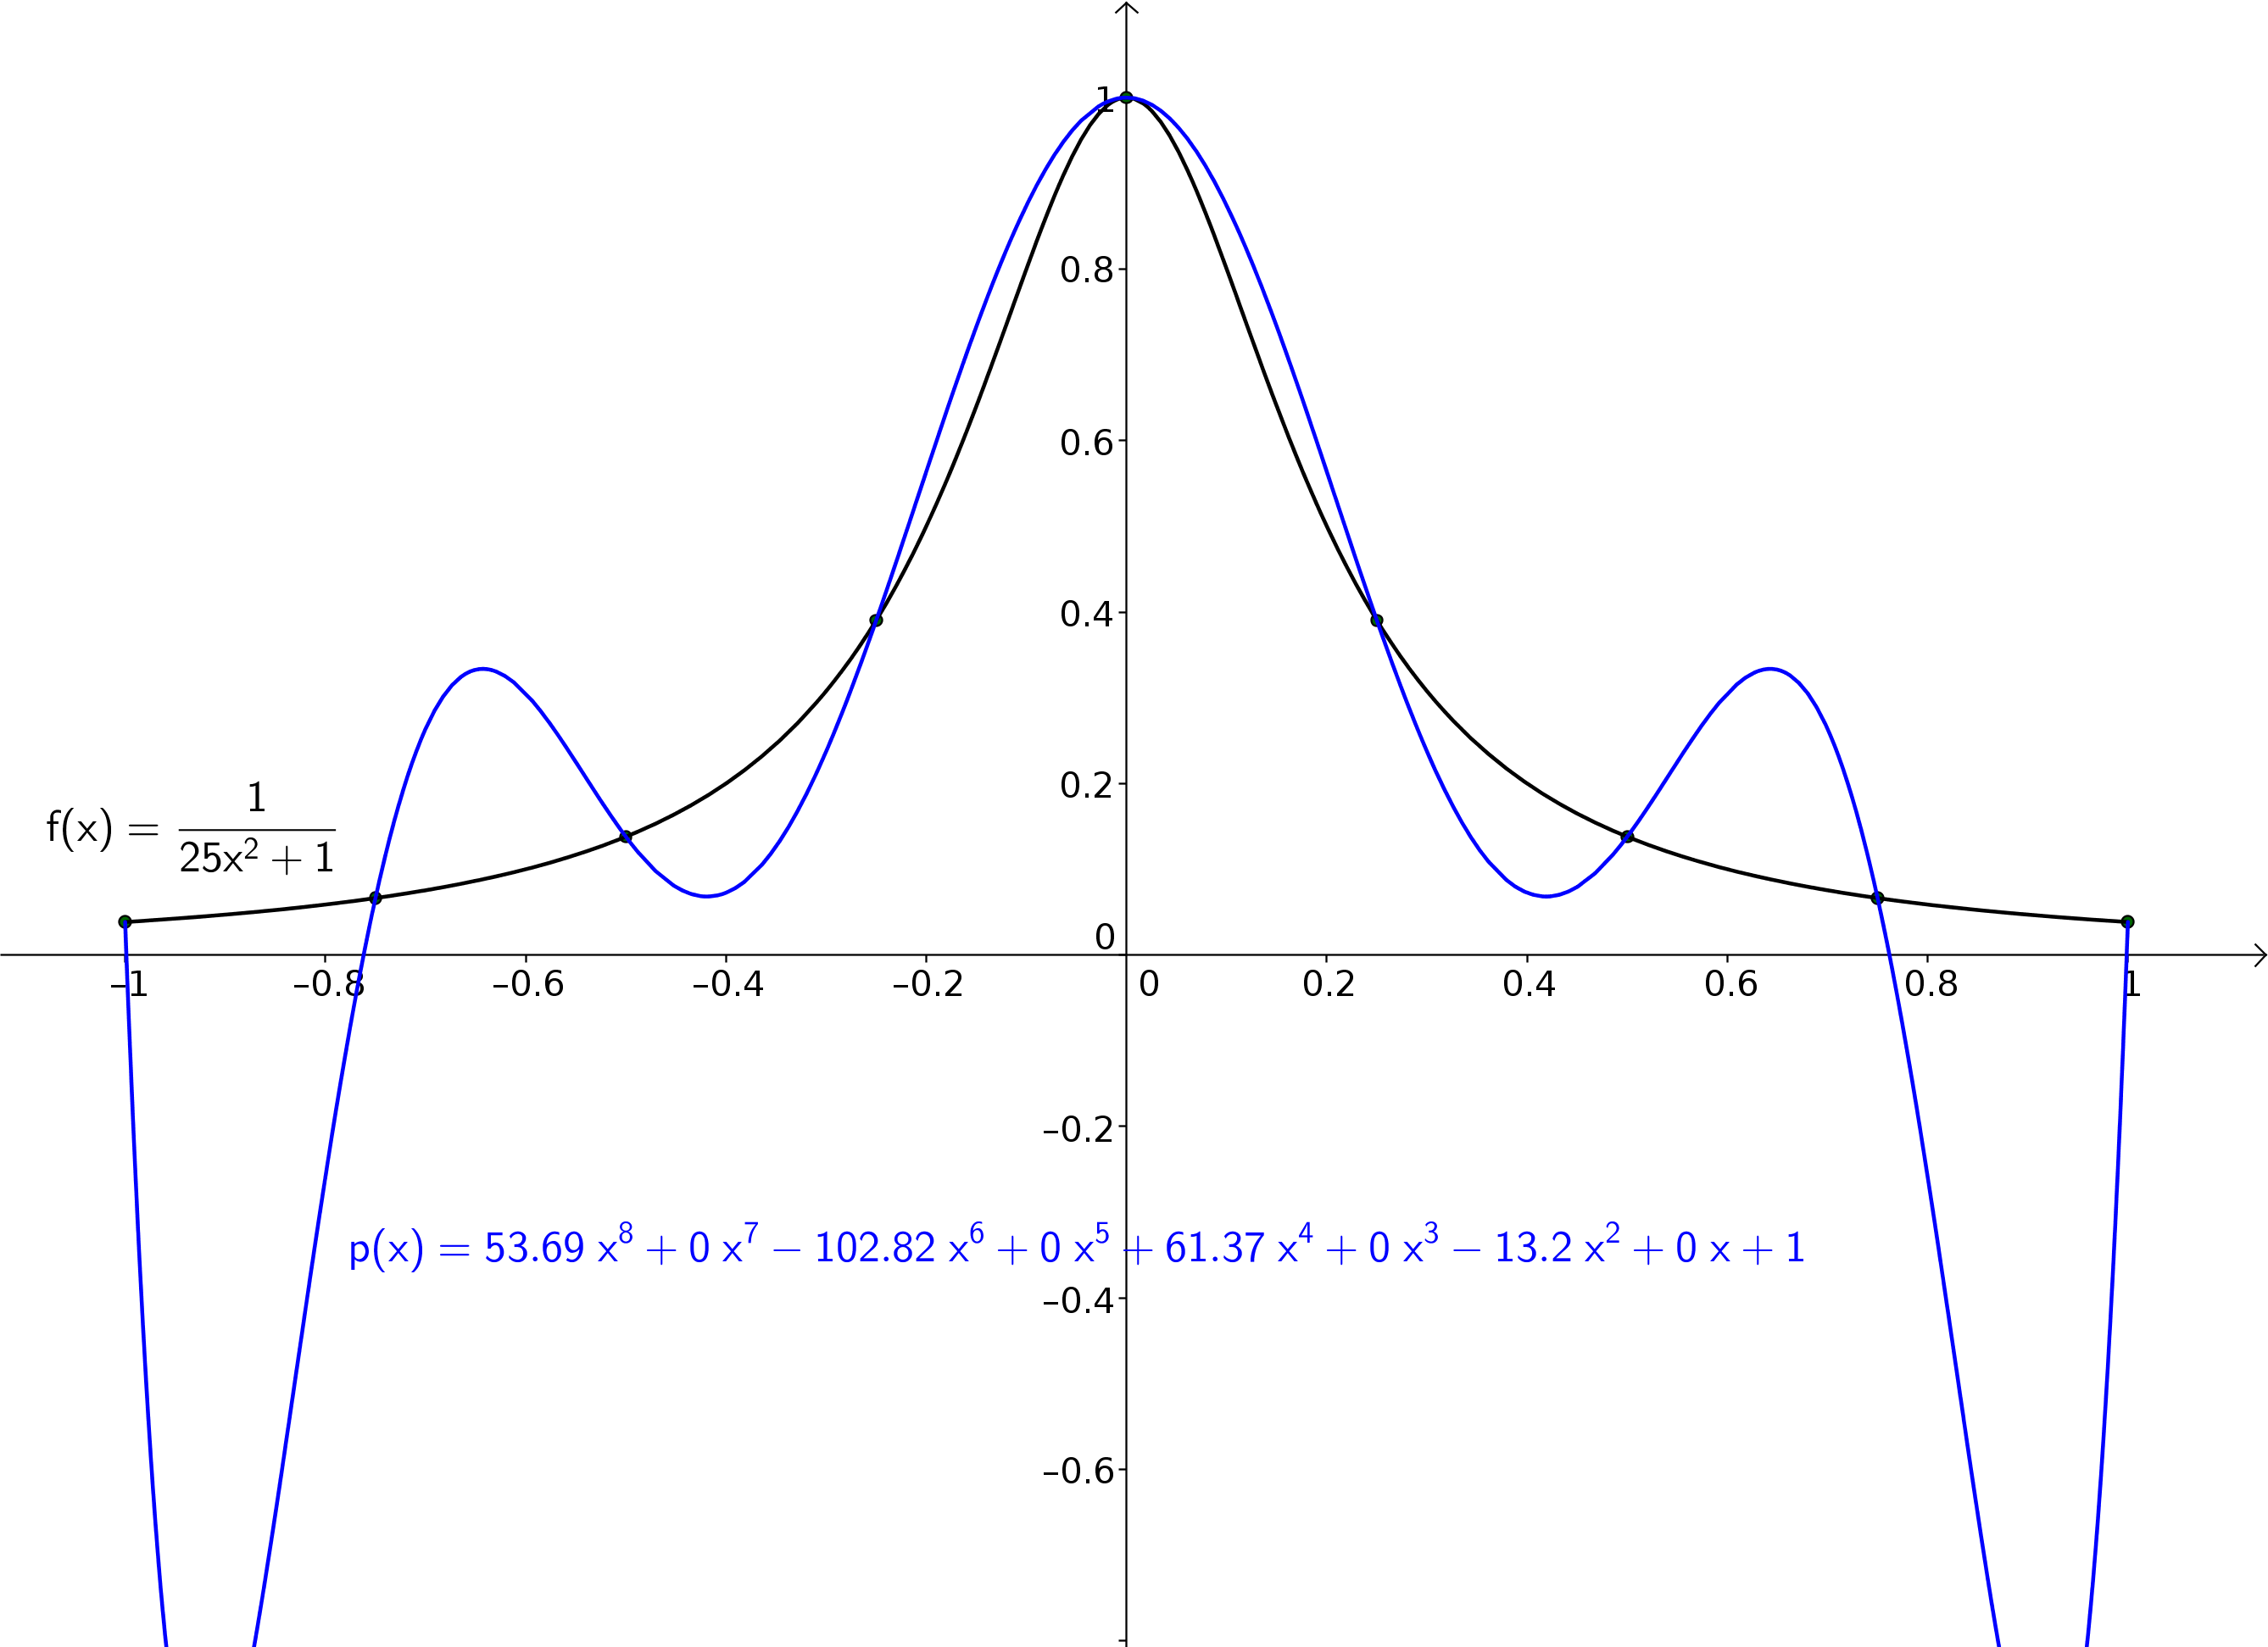
\includegraphics[width=11cm]{./vond_bruun1.png}
 % vond_bruun.png: 806x370 pixel, 96dpi, 21.32x9.79 cm, bb=0 0 604 277
\end{center}

\end{frame}

\begin{frame}{5.4 Um val á brúunarpunktum}
\begin{block}{}
 Það er ekki sjálfgefið að við getum valið í hvaða brúunarpunkta við notum, t.d.~ef þeir 
 ákvarðast af mælingum. \pause Ef við hins vegar getum valið þá óhindrað, þá vaknar sú spurning 
 hvernig er best að gera það?\pause
 
 Fyrst þurfum við að útskýra betur hvað við eigum við með ,,best''. \pause
 Við munum bara notast við tvær leiðir hér til að mæla skekkjuna, en það er 
 $\ell_\infty$ og $\ell_2$ staðlarnir, \pause fyrir samfellt fall 
 $h$ á bilinu $[a,b]$ þá eru þeir skilgreindir með 
 $$
  \|h\|_\infty  = \max_{x\in[a,b]} |h(x)|,
 $$
 \pause og
 $$
  \|h\|_2 = \left( \int_a^b h(x)^2\, dx \right)^\frac 12
 $$
\end{block}
\end{frame}
 
\begin{frame}{5.4 Verkefnið}
Verkefnið er því eftirfarandi: Fyrir gefið fall $f(x)$ á bili $[a,b]$ og 
fast $n$, þá viljum við finna $x_0,\ldots,x_n$ sem lágmarka annað hvort
$$
  \|f-p\|_\infty \quad \text{ eða } \quad \|f-p\|_2.
$$
Þar sem  $p$ er brúunarmargliðan fyrir brúunarpunktana $(x_i,f(x_i))$.

\pause

Byrjum á að skoða $\ell_\infty$ tilvikið. 
 
\end{frame}

\begin{frame}{5.4 Chebyshev margliðurnar}
 \begin{block}{Skilgreining}
  Fyrir náttúrlega tölu $n$ þá skilgreinum við \emph{Chebyshev margliðuna}
  $T_n$ á $[-1,1]$ með 
  $$
    T_n(x) = \cos(n \arccos(x)).
  $$
 %\end{block}
 \pause
 %\begin{block}{}
 Með því að setja inn $n=0$ og $n=1$ þá fæst að 
 $$
  T_0(x) = 1 \quad \text{ og } \quad T_1(x) = x,
 $$
\pause og með hornafallareglunum fæst að 
  $$
    T_{n+1}(x) = 2xT_n(x) - T_{n-1}(x), n \geq 1.
  $$
 %\end{block}
\pause
 %\begin{block}{}
 Af jöfnunni hér á undan þá fæst með þrepun að \pause
  \begin{itemize}
   \item $T_n(x)$ er margliða af stigi $n$.\pause
   \item Forystustuðull $T_n$ er $2^{n-1}$.\pause
   \item $T_n$ er jafnstæð ef $n$ er slétt og oddstæð ef $n$ er oddatala.
  \end{itemize}

 \end{block}
\end{frame}

\begin{frame}{5.4 Chebyshev margliðurnar, framh.}
 \begin{block}{Setning}
  Chebyshev margliðan $T_n$ hefur $n$ einfaldar núllstöðvar á bilinu $[-1,1]$ \pause
  og þær eru gefnar með 
  $$
    x_j = \cos\left(\frac{2j+1}{2n}\pi\right),\qquad j=0,1,2,3,\ldots,n-1.
  $$\pause
  Auk þess eru útgildi $T_n$ á $[-1,1]$ staðsett í 
  $$
    z_j = \cos\left( \frac{j\pi}{n}\right),\qquad j=0,1,2,\ldots,n,
  $$
  \pause og fallgildin þar uppfylla $T_n(z_j) = (-1)^j$
 \end{block}

\end{frame}

\begin{frame}{5.4 Staðlaðar Chebyshev margliður}
 \begin{block}{Skilgreining}
  Margliða er kölluð \emph{stöðluð} ef forystustuðull hennar er 1.
 \end{block}
 \pause
 \begin{block}{Skilgreingin}
  \emph{Stöðluðu Chebyshev margliðurnar} $\tilde T$ eru skilgreindar á eftirfarandi hátt
  $$
    \tilde T(x) = 
    \begin{cases} 
      T_0(x) & \text{ef } n = 0 \\
      2^{1-n}T_n(x)   & \text{ef } n\geq 1      %
        \end{cases}
   $$
 \end{block}
 \pause
 \begin{block}{Setning}
  Fyrir sérhverja staðlaða margliðu $q$ af stigi $n$ þá er 
  $$
    \frac 1{2^{n-1}} = \max_{x\in [-1,1]} T_n(x) \leq \max_{x\in[-1,1]} |q(x)|.
  $$
  \pause
  Þ.e.~af öllum stöðluðum margliðum þá eru stöðluðu Chebyshev margliðurnar ,,minnstar'' 
  á bilinu $[-1,1]$.
 \end{block}
\end{frame}

\begin{frame}{5.4 Skynsamlegir skiptipunktar}
\begin{block}{Skekkjumat}
  Við vitum að skekkjan í því að nálga fallið $f$ með brúunarmargliðu $p$
  með brúunarpunkta $x_0,\ldots,x_n$ er
  $$
    f(x)-p(x) = \frac{f^{(n+1)}(\xi)}{(n+1)!}\, (x-x_0)(x-x_1)\cdots (x-x_n),
  $$
  þar sem $\xi$ er á minnsta bilinu sem inniheldur $x$ og $x_0,x_1,\ldots,x_n$. 
\end{block} \pause
\begin{block}{}
 Ef við skoðum jöfnuna að ofan þá sjáum við að þar sem $n$ og $f$ (og þar með $f^{(n+1)}$) er fast
 þá er stæðan $(x-x_0)\cdots(x-x_n)$ það eina sem við höfum einhverja stjórn á. \pause
 
 Með því að nota Chebyshev margliðurnar þá getum við lágmarkað þennan hluta skekkjunnar.
\end{block}

\end{frame}
  
\begin{frame}{5.4 Skynsamlegir skiptipunktar fyrir bilið $[-1,1]$}

\begin{block}{}
Athugið að $(x-x_0)\cdots (x-x_n)$ er stöðluð margliða af stigi $n+1$. Þannig að skv.~glæru 5.48 
þá lágmörkum við  framlag hennar til skekkjunnar með $(x-x_0)\cdots (x-x_n) = \tilde T_{n+1}$, \pause
þ.e.~með því að velja 
$$
x_i = \cos\left(\frac{2i+1}{2(n+1)}\pi\right), \qquad i=0,1,\ldots,n.
$$
\pause 
Hæsta gildi $\tilde T_{n+1}$ er $\frac 1{2^n}$, sem þýðir að við fáum skekkjumatið
$$
\|f(x)-p(x)\|_\infty \leq \frac{\|f^{(n+1)}\|_\infty}{2^n(n+1)!}.
$$
\end{block}
\end{frame} 


\begin{frame}{5.4 Dæmi um óheppilega skiptipunkta skoðað aftur}
Skoðum aftur fallið 
$f(x) = 1/(25x^2+1)$, en í stað þess að taka 9  jafndreifaða brúunarpunkta
á bilinu $[-1,1]$, þá skulum við nota Chebyshev margliðurnar til að finna 9
punkta á bilinu.

\begin{center}
 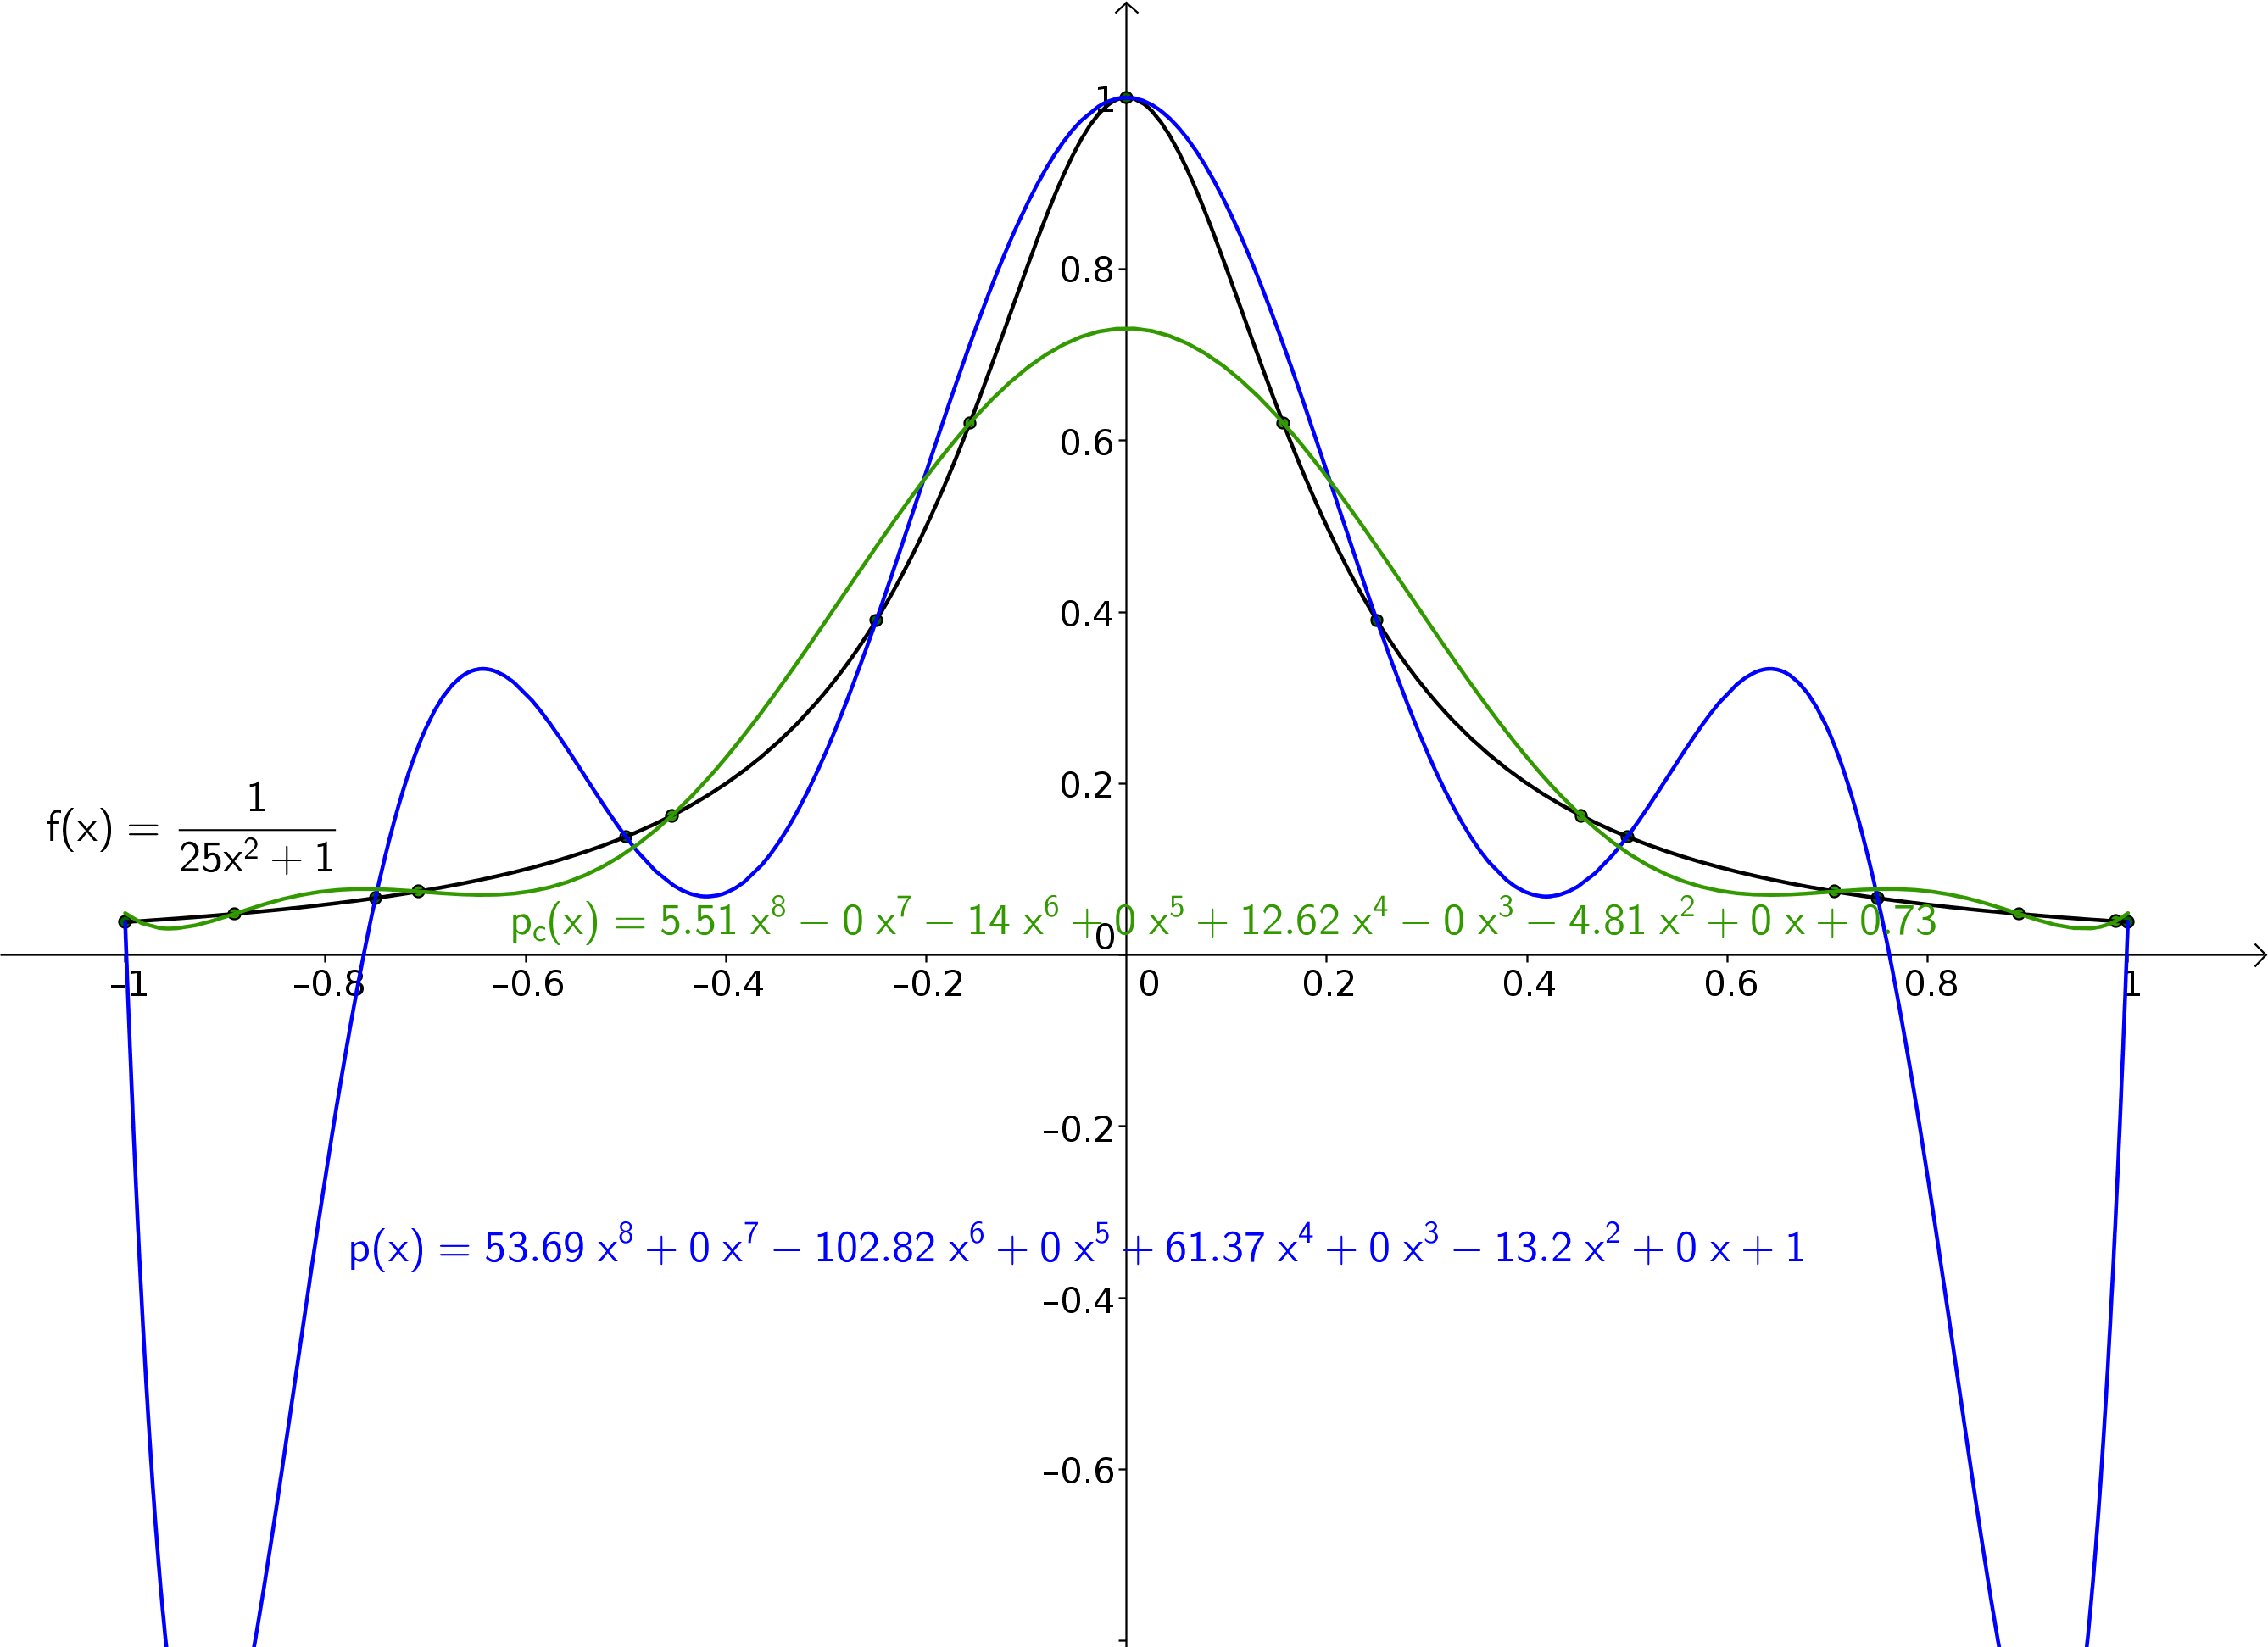
\includegraphics[width=11cm]{./vond_bruun2.png}
 % vond_bruun.png: 806x370 pixel, 96dpi, 21.32x9.79 cm, bb=0 0 604 277
\end{center}

\end{frame}

\begin{frame}{5.4 Skynsamlegir skiptipunktar fyrir bil $[a,b]$}
 \begin{block}{}
  Hér á undan miðaðist allt við að finna brúunarmargliðu fyrir fallið $f$ á bilinu
  $[-1,1]$. \pause
  Ef við viljum skoða almennt bil $[a,b]$ þá byrjum við á athuga að fallið 
  $\eta:[-1,1]\to [a,b]$, 
  $$
    \eta(t) = \frac{b-a}2 t + \frac{b+a}2
  $$
  skilgreinir línulega vörpun (hliðrun og stríkkun) frá $[-1,1]$ yfir á 
  $[a,b]$. \pause
  Athugið að vörpunin sendir $-1$ í $a$ og $1$ í $b$.
  \pause
  
  Með því að taka rætur stöðluðu Chebyshev margliðunnar $\tilde T_{n+1}$ 
  og varpa þeim með $\eta$ yfir á bilið $[a,b]$ þá fáum við þá punkta
  $x_0,\ldots,x_n \in [a,b]$ sem lágmarka 
  $(x-x_0)\cdots (x-x_n)$ á bilinu $[a,b]$,\pause
  $$
    x_i = \eta\left(\cos\left(\frac{2i+1}{2(n+1)}\pi\right)\right) 
    = \frac{b-a}2 \cos\left(\frac{2i+1}{2(n+1)}\pi\right) + \frac{b+a}2,
  $$
  $i=0,1,2,\ldots,n$.
 \end{block}

\end{frame}


\begin{frame}{5.4 Lágmörkun á skekkju með tilliti til $\ell_2$}
 Nú skulum við skipta um staðal, þannig að í stað þess að lágmarka
 $\|f-p\|_\infty$ þá skulum við reyna að lágmarka
 $$
  \|f-p\|_2 = \left(\int_a^b (f-p)^2\, dx\right)^{1/2}
 $$
\pause 

  Við vitum að skekkjan í því að nálga fallið $f$ með brúunarmargliðu $p$
  með brúunarpunkta $x_0,\ldots,x_n$ er
  $$
    f(x)-p(x) = \frac{f^{(n+1)}(\xi)}{(n+1)!}\, (x-x_0)(x-x_1)\cdots (x-x_n),
  $$
  þar sem $\xi$ er á minnsta bilinu sem inniheldur $x$ og $x_0,x_1,\ldots,x_n$. \pause
  
  Eins og áður þá sjáum við að stæðan $(x-x_0)\cdots(x-x_n)$ það eina sem við getum stjórnað
  með því að velja brúunarpunktana $x_j$.

 \end{frame}

\begin{frame}{5.4 Legendre margliðurnar}
 \begin{block}{Skilgreining}
  Fyrir náttúrlega tölu $n$ þá skilgreinum við \emph{Legendre margliðurnar} svona
  \begin{align*}
   P_0(x) &= 1,\\
   P_1(x) &= x,\\
   P_n(x) &= \frac{2n-1}n x P_{n-1}(x) - \frac{n-1}n P_{n-2}(x).
  \end{align*}

 %\end{block}
 \pause
 
 %\begin{block}{}
 Af skilgreiningunni hér á undan þá sjáum við að \pause
  \begin{itemize}
   \item $P_n(x)$ er margliða af stigi $n$.\pause
   \item Forystustuðull $P_n$ er $\frac {2n-1}n \cdot \frac {2n-3}{n-2} \cdots \frac 32 \cdot 1$.\pause
   \item $P_n$ er jafnstæð ef $n$ er slétt og oddstæð ef $n$ er oddatala.
  \end{itemize}

 \end{block}
\end{frame}

\begin{frame}{5.4 Legendre margliðurnar, framh.}
 \begin{block}{Setning}
  $$
    \int_{-1}^1 P_j(x) P_k(x)\, dx =
    \begin{cases}
     0, & \text{ef } j\neq k\\
     \frac{2}{2j+1}, & \text{ef } j=k.
    \end{cases}
  $$
 \end{block}
 \pause
 \begin{block}{Setning}
  Ef $q$ er margliða af stigi minna en $n$ þá er 
  $$
   \int_{-1}^1 q(x)P_n(x)\, dx = 0.
  $$
 \end{block}
\pause
 Þetta segir okkur að Legendre margliðurnar eru hornréttar (með tilliti til innfeldisins sem
 heildið skilgreinir).
 
 \begin{block}{Setning}
  $P_n$ hefur $n$ ólíkar núllstöðvar sem liggja allar á $[-1,1]$.
 \end{block}
  \end{frame}

\begin{frame}{5.4 Staðlaðar Legendre margliður}
 \begin{block}{}
 Eins og þegar við fengumst við Chebyshev margliðurnar þá skilgreinum við 
 \emph{stöðluðu Legendre margliðurnar} $\tilde P_n$ með því að deila upp í $P_n$ með forrystustuðlunum
 $P_n$.
 \end{block}
 \pause
 \begin{block}{Athugasemd}
  Setningarnar þrjár hér undan gilda um $\tilde P$ alveg eins og $P$.
 \end{block}
 \end{frame}
 \begin{frame}{5.4 Lágmörkunareiginleikar Legendre margliðanna}
 \begin{block}{Setning}
 Ef $p$ er stöðluð margliða af stigi $n+1$ þá er $\|p\|_2\geq \|\tilde P_{n+1}\|_2$.
 \end{block}\pause
 \begin{block}{Sönnun}
  Skilgreinum $q = p-\tilde P_{n+1}$, sem þýðir að $q$ er margliða af stigi minna en $n+1$. \pause
  Nú er 
  \begin{align*}
   \|p\|_2^2 &= \|\tilde P_{n+1} + q\|_2^2 \\
   &= \int_{-1}^1 (\tilde P_{n+1}(x) + q(x))^2\, dx \\
   &= \int_{-1}^1 \tilde P_{n+1}(x)^2 + 2q(x)\tilde P_{n+1}(x) + q(x)^2\, dx\\
   &= \|\tilde P_{n+1}\|_2^2 + 2\int_{-1}^1 q(x)\tilde P_{n+1}(x)\, dx + \|q\|_2^2\\
   &= \|\tilde P_{n+1}\|_2^2 +  \|q\|_2^2 \geq \|\tilde P_{n+1}\|_2^2
  \end{align*}
  því $\int_{-1}^1 q(x)\tilde P_{n+1}(x)\, dx=0$ og $\|q\|_2 \geq 0$.
 \end{block}
\end{frame}

 \begin{frame}{5.4 Lágmörkun með Legendre margliðunum}
  Af síðustu setningu sjáum við að til þess að lágmarka 
  $$
      \|f(x)-p(x)\|_2 = \left\|\frac{f^{(n+1)}(\xi)}{(n+1)!}\, (x-x_0)(x-x_1)\cdots (x-x_n) \right\|_2,
  $$
  þá veljum við $x_1,\ldots,x_n$ þannig að 
  $(x-x_0)(x-x_1)\cdots (x-x_n) = \tilde P_{n+1}$. Þ.e.~$x_j$ þurfa að vera rætur 
  stöðluðu Legendre margliðunnar af stigi $n+1$.
  \pause
  
  Ólíkt Chebyshev margliðunum þá er ekki hlaupið að því að finna rætur $\tilde P_{n+1}$.
  Þannig að við þurfum að reikna þær tölulega og geyma í töflu.
  \end{frame}
  
  \begin{frame}{5.4 Núllstöðvar $P_n$, fyrir $n=1,\ldots,10$}
  \begin{center}
 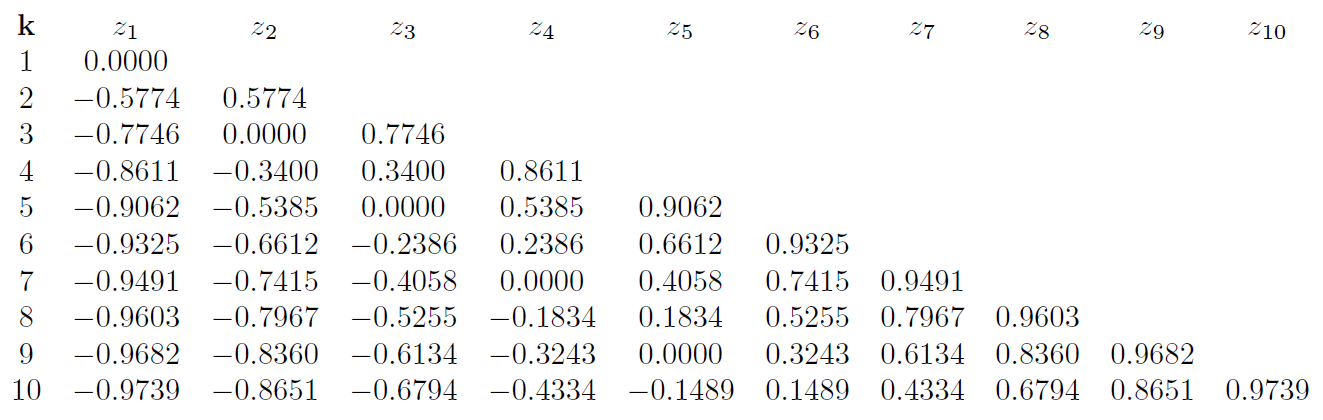
\includegraphics[width=11.8cm]{./legendre.png}
 % legendre.png: 1323x420 pixel, 96dpi, 35.01x11.11 cm, bb=0 0 992 315
\end{center}

 \end{frame}

 \begin{frame}{5.4 Dæmi um óheppilega skiptipunkta skoðað aftur}
Skoðum enn einu sinni fallið 
$f(x) = 1/(25x^2+1)$, en í stað þess að taka 9  jafndreifaða brúunarpunkta
á bilinu $[-1,1]$, þá skulum við nota Legendre margliðurnar til að finna 9
punkta á bilinu.  
\begin{center}
 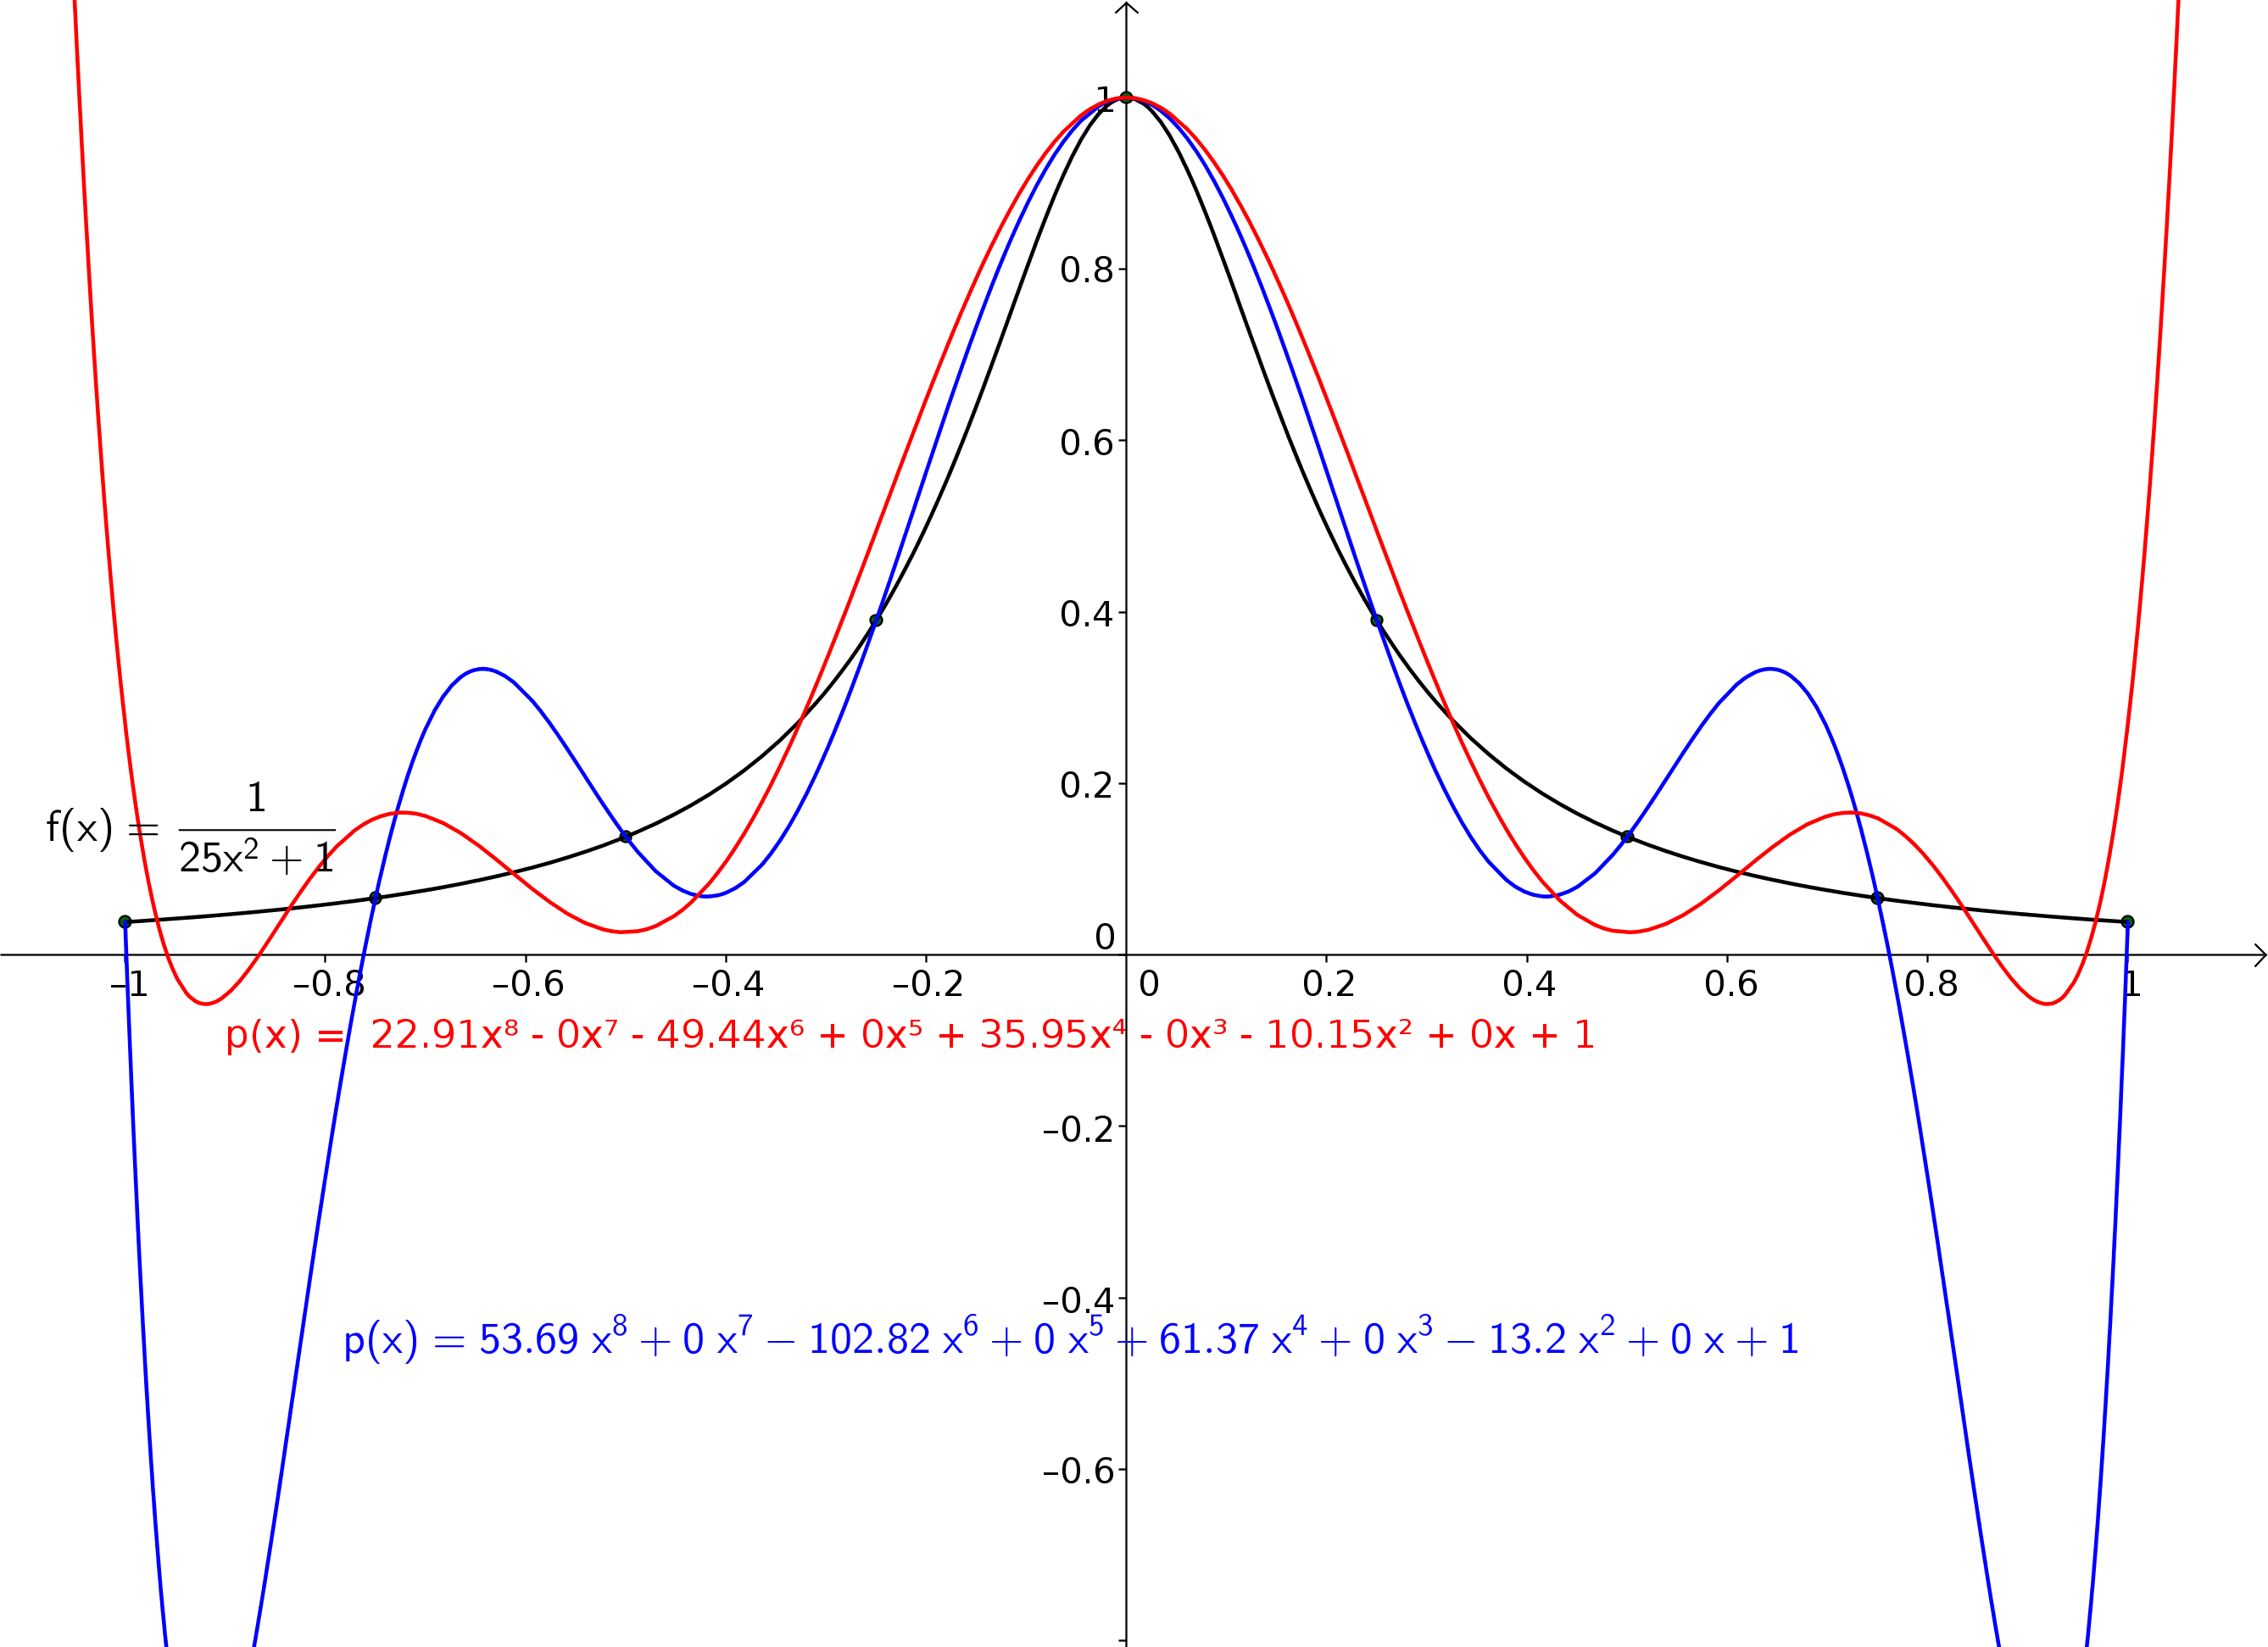
\includegraphics[width=11cm]{./vond_bruun3.png}
 % vond_bruun.png: 806x370 pixel, 96dpi, 21.32x9.79 cm, bb=0 0 604 277
\end{center}

\end{frame}


\begin{frame}{5.4 Athugasemd um $\ell_\infty$ og $\ell_2$}
\begin{block}{$\ell_\infty$}
 Athugið að þegar við notum $\ell_\infty$ og Chebyshev margliðurnar þá erum við 
 að reyna að lágmarka mestu skekkju á bilinu. 
 \end{block}\pause
 
 \begin{block}{$\ell_2$}
 En þegar við notum $\ell_2$ og Legendre margliðurnar þá erum við að reyna að 
 lágmarka heildi skekkjunnar, þ.e.~í einhverjum skilningi, flatarmálið á milli 
 fallsins $f$ og brúunarmargliðunnar okkar.
 \end{block}
\end{frame}

%%%%%%%%%%%%%%%%%%%%%%%%%%%%%%%%%%%%%%%%%%%%%%%%%%%
\section*{Nálgun á föllum með margliðum og skekkjumat}
%%%%%%%%%%%%%%%%%%%%%%%%%%%%%%%%%%%%%%%%%%%%%%%%%%%

%%%%%%%%%%%%%%%%%%%%%%%%%%%%%%%%%%%%%%%%%%%%%%%%%%%
\begin{frame}{5.1  Nálgun á föllum með margliðum} 
Lítum nú aftur á almenna brúunarverkefnið og
gefum okkur að  tölurnar $y_i^{(j)}$ séu af gerðinni $f^{(j)}(a_i)$ 
þar sem $f : I \to \R$ er fall á bili $I$ sem inniheldur alla
punktana  $a_1, \ldots, a_k$.

\pause
\smallskip
Þá snýst brúunarverkefnið um að finna
margliðu  af stigi $\leq m$ sem uppfyllir
\begin{equation*}
  p^{(j)}(a_i) = f^{(j)}(a_i), \quad
  j = 0, \ldots, m_i-1, \quad i = 1, \ldots, k.
\end{equation*}

\pause
\smallskip
Við vitum að lausn þess er ótvírætt ákvörðuð.  Ef við notum Newton
form lausnarinnar, þá táknum við mismunakvótana með
$$
f[x_i,\ldots,x_{i+j}]
$$
í stað 
$$
y[x_i,\ldots,x_{i+j}]
$$
\end{frame}

%%%%%%%%%%%%%%%%%%%%%%%%%%%%%%%%%%%%%%%%%%%%%%%%%%%
\begin{frame}{5.1 Nálgun á fallgildum} 
Runurnar $(x_0,\ldots,x_m)$ og 
$(y_0,\ldots,y_m)$ eru skilgreindar með 
\begin{equation*}
  (x_0,x_1,\ldots,x_m) = 
  (\underbrace{a_1, \ldots, a_1}_{m_1 \, \text{sinnum}}, 
  \underbrace{a_2, \ldots , a_2}_{m_2 \, \text{sinnum}}, 
  \ldots , 
  \underbrace{a_k, \ldots , a_k}_{m_k \, \text{sinnum}}) 
\end{equation*}
og
\begin{multline*}
  (y_0,y_1,\ldots,y_m) = 
  (f^{(0)}(a_1), \ldots, f^{(m_1-1)}(a_1),
f^{(0)}(a_2), \ldots, f^{(m_2-1)}(a_2) \\ \ldots,
  f^{(0)}(a_k), \ldots, f^{(m_k-1)}(a_k))
  \label{bru.margfald.5}
\end{multline*}
\end{frame}

%%%%%%%%%%%%%%%%%%%%%%%%%%%%%%%%%%%%%%%%%%%%%%%%%%%
\begin{frame}{5.1 Skekkjumat} 
Nú tökum við punkt $x \in I$ og spyrjum um skekkjuna 
$f(x) - p(x)$ í nálgun á $f(x)$ með $p(x)$. Ef $x$ er einn punktana 
$a_1, \ldots, a_k$, þá er $p(x) = f(x)$ og skekkjan þar með 0, svo 
við skulum gera ráð fyrir að $x \not= a_i$, $i = 1, \ldots, k$.

\pause
\smallskip
Við bætum nú $(x,f(x))$ sem einföldum brúunarpunkti við
alhæfða brúunar verkefnið  og fáum sem lausn $q(t)$ á þessu aukna verkefni. 
Margliðan $q$ er af stigi $\leq m+1$. Við notum táknið $t$ fyrir 
breytu, því $x$ er frátekið. 

\pause
\smallskip
Þá uppfyllir $q(t)$ að $q(x) = f(x)$ 
auk allra skilyrðanna 
$$
q^{(j)}(a_i) = p^{(j)}(a_i) = f^{(j)}(a_i)
$$ 
í verkefninu sem við byrjuðum með.
\end{frame}

%%%%%%%%%%%%%%%%%%%%%%%%%%%%%%%%%%%%%%%%%%%%%%%%%%%
\begin{frame}{5.1 Skekkjumat} 
Við getum þá skrifað (sjá glæru 5.27 til hliðsjónar)
\begin{align*}
  q(t) &= p(t) + f[x_0,\ldots,x_m,x](t-x_0)\cdots(t-x_m) \\
  &= p(t) + f[x_0,\ldots,x_m,x](t-a_1)^{m_1}\cdots(t-a_k)^{m_k}.
\end{align*}

\pause
Þegar við gefum breytunni $t$ gildið $x$, þá fáum við $q(x) = f(x)$
og  því fæst formúla fyrir skekkjunni
\begin{equation*}
  f(x) - p(x) 
  = f[x_0,\ldots,x_m,x](x-a_1)^{m_1}\cdots(x-a_k)^{m_k}
\end{equation*} 

\pause
Nú ætlum við að finna leið til þess að meta skekkjuliðinn. 
Til þess þurfum við að gefa okkur að $f$ hafi að minnsta kosti 
$m+1$ afleiðu.
\end{frame}

%%%%%%%%%%%%%%%%%%%%%%%%%%%%%%%%%%%%%%%%%%%%%%%%%%%
\begin{frame}{5.1 Tilfellið þegar við höfum aðeins einn punkt} 
Munum nú að í tilfellinu þegar við erum bara með einn punkt 
$a_1$, þá erum við með $m+1$ skilyrði 
$$p^{(j)}(a_1)=f^{(j)}(a_1), \qquad j=0,\dots,m
$$
og við fáum að $p$ er Taylor-margliða fallsins $f$ í punktinum $a_1$.
Þá er $x_0=\cdots=x_m=a_1$ og við fáum
\begin{equation*}
  f(x) - p(x) 
  = f[x_0,\ldots,x_m,x](x-a_1)^{m+1}
\end{equation*} 

\pause
Nú segir setning Taylors okkur að til sé punktur $\xi$ milli $a_1$ og
$x$ þannig að 
$$
  f(x) - p(x) 
  = \dfrac{f^{(n+1)}(\xi)}{(n+1)!}(x-a_1)^{m+1}
$$
Við getum því dregið þá ályktun að í þessu sértilfelli er
$$
f[x_0,\ldots,x_m,x]=\dfrac{f^{(n+1)}(\xi)}{(n+1)!}
$$
Það kemur í ljós að þetta er almenn regla sem gildir
fyrir {\it öll} alhæfðu brúunarverkefnin.
\end{frame}

%%%%%%%%%%%%%%%%%%%%%%%%%%%%%%%%%%%%%%%%%%%%%%%%%%%
\begin{frame}{5.1 Tilfellið $m=1$ er meðalgildisreglan} 
Munum að tilfellið $m=1$ er meðalgildisreglan
$$
f[a_1,x]=\dfrac{f(x)-f(a_1)}{x-a_1}=f'(\xi).
$$
\end{frame}

\begin{frame}{5.1 Margfeldni núllstöðva:} 

Samfellt fall $\varphi$ á bili $I$ er sagt hafa núllstöð {\it af stigi 
að minnsta kosti $m>0$} í punktinum $a\in I$, ef til er samfellt fall 
$\psi$ á $I$ þannig að 
$$
\varphi(x)=(x-a)^m\psi(x)
$$   
Við segjum að $\varphi$ hafi núllstöð af {\it margfeldni} $m$ ef
$\psi(a)\neq0$.

\pause
\smallskip
Athugið að ef $\varphi$ er deildanlegt  $I$ með samfellda afleiðu, 
þá er $\psi$ deildanlegt með samfellda afleiðu í $I\setminus\{a\}$ og 
við höfum
\begin{align*}
  \varphi'(x)&=m(x-a)^{m-1}\psi(x)+(x-a)^m\psi'(x)\\
&= (x-a)^{m-1} \big(m\psi(x)+(x-a)\psi'(x)\big)
\end{align*}
Ef afleiðan $\psi'$ er takmörkuð í grennd um $a$, þá sjáum við á
þessari formúlu að 
$\varphi'$ hefur núllstöð af stigi að minnsta kosti $m-1$ í $a$.
\end{frame}

%%%%%%%%%%%%%%%%%%%%%%%%%%%%%%%%%%%%%%%%%%%%%%%%%%%
\begin{frame}{5.1 Núllstöðvar taldar með margfeldni} 
Hugsum okkur nú að við séum með $a_1,\dots,a_k$ ólíka punkta í bilinu 
$I$  og að $m_1,\dots,m_k$ séu jákvæðar náttúrlegar tölur.

\pause
Ef fallið $\varphi$ hefur núllstöðvar í öllum punktunum $a_j$ og 
núllstöðin $a_j$ er af stigi að minnsta kosti $m_j$.  Við segjum að þá
hafi $\varphi$ {\it að minnsta kosti} 
$$
n=m_1+\cdots+m_k
$$
{\it núllstöðvar taldar með margfeldni}.

\pause
\smallskip
Eins þá segjum við að  $\varphi$ hafi $n$ núllstöðvar í $\{a_1,\dots,a_k\}$ 
{\it taldar með margfeldni} ef $\varphi$ hefur 
núllstöðvar í öllum punktum $a_1,\dots,a_k$ og samanlögð margfeldni
þeirra er  $n$
\end{frame}

%%%%%%%%%%%%%%%%%%%%%%%%%%%%%%%%%%%%%%%%%%%%%%%%%%%
\begin{frame}{5.1 Margfeldni núllstöðva} 
Hugsum okkur nú að fallið $\varphi$ hafi núllstöð af stigi 
$m_j$ í punktunum $a_j$ fyrir öll $j=1,\dots,k$ og að
$n=m_1+\cdots+m_k$.  

\pause
\smallskip
Til einföldunar gerum við ráð fyrir að 
$$
a_1<a_2<\cdots<a_k.
$$

\pause
\smallskip
Þá gefur meðalgildissetningin að $\varphi'$ hefur að minnsta kosti eina
núllstöð á sérhverju bilanna 
$$
]a_1,a_2[, \  ]a_2,a_3[, \ \dots \  ]a_{k-1},a_k[ 
$$
Þau eru samanlagt $k-1$ talsins.  Að auki vitum við að 
$\varphi'$ hefur núllstöðvar af stigi að minnsta kosti 
$m_j-1$ í punktinum $a_j$.   Ef við leggjum þetta saman, þá fáum við
að $\varphi'$ hefur núllstöðvar af margfeldni að minnsta kosti 
$$
k-1+(m_1-1)+\cdots+(m_k-1)=n-1
$$
í minnsta lokaða bilinu sem inniheldur alla punktana $a_1,\dots,a_k$.  
\end{frame}

%%%%%%%%%%%%%%%%%%%%%%%%%%%%%%%%%%%%%%%%%%%%%%%%%%%
\begin{frame}{5.1 Skekkjumat -- aftur} 
Nú ætlum við að sýna fram á að fyrir föll $f$ sem eru $(m+1)$ sinnum 
samfellt deildanleg að til sé $\xi$ á minnsta bili sem inniheldur 
$a_1, \ldots, a_k$ og $x$ þannig að
\begin{equation*}
  f[x_0,\ldots,x_m,x] = \frac{f^{(m+1)}(\xi)}{(m+1)!}
\end{equation*}

\pause
\smallskip
Við skilgreinum fallið
\begin{equation*}
  g(t) = f(t) - p(t) - \lambda w(t),
\end{equation*}
þar sem
\begin{equation*}
  w(t) = (t-a_1)^{m_1} \cdots (t-a_k)^{m_k}
\end{equation*}
og talan $\lambda$ er valin þannig að $g(x) = 0$. 

\pause
\smallskip
Nú er $p^{(j)}(a_i)=f^{(j)}(a_i)$  fyrir $j=0,\dots,m_i-1$,   
þá gefur setning Taylors okkur að $g$
hefur núllstöð  af stigi $m_i$ í sérhverjum punktanna $a_i$.
Auk þess hefur $g$ núllstöð í $x$.  Samanlagt eru þetta  að minnsta
kosti 
$m+2$ núllstöðvar taldar með margfeldni.
\end{frame}

%%%%%%%%%%%%%%%%%%%%%%%%%%%%%%%%%%%%%%%%%%%%%%%%%%%
\begin{frame}{5.1 Skekkjumat -- aftur} 
 Höfum:

\smallskip
$g$ hefur  að minnsta kosti $m+2$ núllstöðvar taldar með margfeldni,

\pause
\smallskip
$g'$ hefur  að minnsta kosti $m+1$ núllstöð talda með margfeldni,


\pause
\smallskip
$g''$ hefur  að minnsta kosti $m$ núllstöðvar taldar með margfeldni 

\pause
\smallskip
og þannig áfram, þar til við ályktum að 


\pause
\smallskip
$g^{(m+1)}$ hefur  að minnsta kosti eina  núllstöð.  

\pause
\smallskip
Tökum eina slíka og köllum $\xi$.
\end{frame}

%%%%%%%%%%%%%%%%%%%%%%%%%%%%%%%%%%%%%%%%%%%%%%%%%%%
\begin{frame}{5.1 Skekkjumat -- aftur} 
Munum að 
\begin{equation*}
  g(t) = f(t) - p(t) - \lambda w(t),
\end{equation*}
þar sem
\begin{equation*}
  w(t) = (t-a_1)^{m_1} \cdots (t-a_k)^{m_k}=t^{m+1}+b_mt^m+\cdots+b_1t+b_0
\end{equation*}

\pause
\smallskip
Margliðan $p$ hefur stig $\leq m$ svo $p^{(m+1)}(x) = 0$  fyrir öll
$x$ 

\pause
og margliðan $w$ er af stigi $m+1$ með stuðul $1$ við hæsta veldið,
svo $w^{(m+1)}(t) = (m+1)!$. Við höfum því
\begin{equation*}
  0 = g^{(m+1)}(\xi) = f^{(m+1)}(\xi) - \lambda \cdot (m+1)!
\end{equation*}
sem jafngildir því að
$$
\lambda =\dfrac{f^{(m+1)}(\xi)}{(m+1)!}
$$
\end{frame}

%%%%%%%%%%%%%%%%%%%%%%%%%%%%%%%%%%%%%%%%%%%%%%%%%%%
\begin{frame}{5.1 ... og nú er þetta loksins búið} 
Við setjum nú inn $t=x$ sem gefur 
\begin{equation*}
0=g(x) = f(x) - p(x) - \lambda w(x),
\end{equation*}
og við fáum þar með formúlu fyrir skekkjunni á nálgun á $f(x)$
með alhæfðu brúunarmargliðunni $p(x)$, 
\begin{equation*}
f(x) - p(x) =\lambda w(x) = \dfrac{f^{(m+1)}(\xi)}{(m+1)!} 
(x-a_1)^{m_1} \cdots (x-a_k)^{m_k}
\end{equation*}
\end{frame}

%%%%%%%%%%%%%%%%%%%%%%%%%%%%%%%%%%%%%%%%%%%%%%%%%%%
\begin{frame}{5.1 Samantekt} 
Ef gefið er fall $f:I\to \R$ á bili $I$, $a_1,\dots,a_k$ í $I$, 
með $a_j\neq a_k$ ef $j\neq k$, jákvæðar heiltölur $m_1,\dots,m_k$,  
talan $m$ er skilgreind með $m=m_1+\cdots+m_k-1$, og gert er ráð fyrir
að $f\in C^{m+1}(I)$, þá er til nákvæmlega ein margliða $p$
af stigi $\leq m$ þannig að
$$
p^{(j)}(a_i)=f^{(j)}(a_i), \qquad j=0,\dots, m_i-1, \quad i=1,\dots,k. 
$$  
\end{frame} 

%%%%%%%%%%%%%%%%%%%%%%%%%%%%%%%%%%%%%%%%%%%%%%%%%%%
\begin{frame}{5.1 Samantekt} 
Newton-form margliðunnar $p$ er gefið með
$$
  p(x)=f[x_0]+f[x_0,x_1](x-x_0)+\cdots+f[x_0,\dots,x_m](x-x_0)\cdots(x-x_{m-1})
$$
þar sem mismunakvótarnir $f[x_i,\dots,x_{i+j}]$ eru skilgreindir sem
$y[x_i,\dots,x_{i+j}]$ út frá gögnunum $y^{(j)}_i$.  Fyrir sérhvert
$x$ í $I$ er skekkjan $f(x)-p(x)$ í nálgun á $f(x)$ með $p(x)$ gefin með
$$
  f(x)-p(x)=f[x_0,\dots,x_m,x](x-a_1)^{m_1}\cdots(x-a_k)^{m_k}.
$$

\pause
Fyrir sérhvert $i=1,\dots,k$ og $j=0,\dots,m-i$ þá gildir að til er
tala $\xi$ á minnsta bilinu sem inniheldur $x_i\dots,x_{i+j}$  þannig
að
$$
  f[x_i,\dots,x_{i+j}]=\dfrac{f^{(j)}(\xi)}{j!},
$$
\end{frame}

%%%%%%%%%%%%%%%%%%%%%%%%%%%%%%%%%%%%%%%%%%%%%%%%%%%
\begin{frame}{5.1 Samantekt} 
því gildir sérstaklega að til er tala $\xi$ á minnsta bilinu sem
inniheldur $a_1,\dots,a_k$ og $x$ þannig að 
$$
f(x)-p(x)=\dfrac{f^{(m+1)}(\xi)}{(m+1)!}(x-a_1)^{m_1}\cdots(x-a_k)^{m_k}.
$$
\end{frame}

%%%%%%%%%%%%%%%%%%%%%%%%%%%%%%%%%%%%%%%%%%%%%%%%%%%
\begin{frame}{5.1 Sýnidæmi} 
Látum $f(x)=x^2\ln x$.  

\smallskip
{\bf a)} \  Setjið upp mismunakvótatöflu til þess að 
reikna út brúunarmargliðu $p$ af stigi $\leq 3$  fyrir fallið $f$, 
sem hefur tvo tvöfalda brúunarpunkta $a_1=1$ og $a_2=2$.
Skrifið upp Newton-form margliðunnar $p$.

\pause
\smallskip
{\bf b)} \  Reiknið út  $p(1.3)$. Notið aðferðarskekkju
fyrir margliðubrúun til þess að meta skekkjuna
$f(1.3)-p(1.3)$ að ofan og neðan og fáið þannig bil
þar sem rétta gildið liggur.  Veljið miðpunkt bilsins
sem nálgunargildi fyrir $f(1.3)$ og afrúnið gildið miðað
við mörk bilsins.

\pause
\smallskip
{\bf c)} \ Látum nú $q$ vera brúnunarmargliðuna
af stigi $\leq 4$  sem uppfyllir sömu skilyrði og gefin eru í {\bf a)}
að viðbættu því að $a_2=2$ á að vera þrefaldur brúunarpunktur.
Sýnið hvernig hægt er að ákvarða  mismunakvótatöfluna fyrir $q$
með því  að stækka töfluna í {\bf a)}.  Ákvarðið síðan $q$ og 
reiknið út $q(1.3)$.
\end{frame}

%%%%%%%%%%%%%%%%%%%%%%%%%%%%%%%%%%%%%%%%%%%%%%%%%%%
\begin{frame}{5.1  Lausn á sýnidæmi} 
{\bf Lausn:}  {\bf a)} (og {\bf c)}).  \ Til þess að spara pláss 
skulum við reikna strax út
mismunakvótatöfluna fyrir fjórða stigs margliðuna í {\bf c)}-lið.
Punktarnir $x_0,\dots,x_4$ eru þá $1,1,2,2,2$ og við höfum gefin
fallgildin 
$$f(1)=f[x_0]=f[x_1]=0 \qquad  \text{ og } \qquad
f(2)=f[x_2]=f[x_3]=f[x_4].
$$

\pause
\smallskip
Í {\bf a)}-lið eru punktarnir tvöfaldir svo við höfum gefin 
gildi afleiðunnar  $f'(x)=2x\ln x+x$ í punktunum $1$ og $2$.
$$
f'(1)=f[1,1]=f[x_0,x_1]=1 \ \text{ og } \  
f'(2)=f[2,2]=f[x_2,x_3]=4\ln 2+2.
$$

\pause
\smallskip
Í {\bf c)}-lið er gildið á 2. afleiðu $f''(x)=2\ln x +3$ gefið
í punktinum $2$.  Það gefur okkur
$$f''(2)/2!=f[2,2,2]=f[x_2,x_3,x_4]=\ln 2+\tfrac 32.
$$   

\pause
Við setjum þessi gildi inn í mismunakvótatöfluna og 
fyllum hana út með því að taka mismunakvóta milli allra gilda 
\end{frame}

%%%%%%%%%%%%%%%%%%%%%%%%%%%%%%%%%%%%%%%%%%%%%%%%%%%
\begin{frame}{5.1 Lausn á sýnidæmi -- framhald} 
$$
\begin{matrix}
i&x_i & f[x_i] &f[x_i,x_{i+1}] & f[x_i,x_{i+1},x_{i+2}] &
f[x_i,\dots,x_{i+3}]&f[x_i,\dots,x_{i+4}] \\\hline
0&1&0     &1       &4\ln 2-1        &-4\ln 2+3& 5\ln 2-\tfrac 72\\
1&1&0     &4\ln 2  &2               &\ln 2-\tfrac 12\\
2&2&4\ln 2&4\ln 2+2&\ln 2+\tfrac 32\\
3&2&4\ln 2&4\ln 2+2\\
4&2&4\ln 2
\end{matrix}
$$

\pause
Margliðan í (a) lið er  
$$p(x)=(x-1)+(4\ln 2-1)(x-1)^2+(-4\ln 2+3)(x-1)^2(x-2).
$$
en í (c)-lið er hún
$$
q(x)=p(x)+(5\ln 2-\tfrac 72)(x-1)^2(x-2)^2
$$
\end{frame}

%%%%%%%%%%%%%%%%%%%%%%%%%%%%%%%%%%%%%%%%%%%%%%%%%%%
\begin{frame}{5.1 Lausn á sýnidæmi -- framhald} 
{\bf b)}  Við stingum gildinu $x=1.3$ inn í margliðuna og fáum
 $p(1.3)=0.445206074$. Skekkjan er
$$
f(x)-p(x)=\dfrac{f^{(4)}(\xi)}{4!}(x-1)^2(x-2)^2
$$ 
þar sem $\xi$ er einhver punktur á bilinu $[1,2]$.

\pause
\smallskip  
Við þurfum því að meta fjórðu afleiðuna,
\begin{align*}
f(x) &=x^2\ln x, \quad
f'(x)=2x\ln x+x, \quad
f''(x)=2\ln x+3, \quad
\\  
f'''(x)& =2/x, \quad
f^{(4)}(x)=-2/x^2.
\end{align*}
Ef $x\in [1,2]$, þá höfum við matið
$-2\leq f^{(4)}(x)\leq -\tfrac 12$. 
\end{frame}

%%%%%%%%%%%%%%%%%%%%%%%%%%%%%%%%%%%%%%%%%%%%%%%%%%%
\begin{frame}{5.1 Lausn á sýnidæmi -- framhald} 
Af ójöfnunum  $-2\leq f^{(4)}(x)\leq -\tfrac 12$
leiðir síðan að
$$
\alpha=\dfrac{-2\cdot(0.3)^2\cdot(-0.7)^2}{24}\leq f(1.3)-p(1.3)
\leq \dfrac{-0.5\cdot(0.3)^2\cdot(-0.7)^2}{24}=\beta.
$$

\pause
\smallskip
 Við reiknum út úr báðum brotunum
$$\alpha=-0.003675 \qquad \text{ og } \qquad 
\beta=-0.00091875.
$$
þar með er $f(1.3)$ á bilinu milli 
$p(1.3)+\alpha=0.441531$ og $p(1.3)+\beta=0.444287$.


\pause
Nálgunargildi okkar á að vera miðpunktur þessa bils og 
algildi skekkjunnar verður þá hálf billengdin.
Það færir okkur nálgunina
$f(1.3) \approx 0.442909$ og skekkjuna $\pm 0.0014$.
Réttur afrúningur er $f(1.3)=0.44$.
\end{frame}

%%%%%%%%%%%%%%%%%%%%%%%%%%%%%%%%%%%%%%%%%%%%%%%%%%%
\begin{frame}{5.1 Lausn á sýnidæmi -- framhald} 
Við eigum aðeins eftir að reikna út gildi 
margliðunnar $q$ í punktinum $1.3$.  Út úr mismunakvótatöflunni
fáum við
$$
q(x)=p(x)+(5\ln 2-\tfrac 72)(x-1)^2(x-2)^2
$$
sem gefur okkur gildið
$$
q(1.3)=0.445206074-0.001511046=0.4436950278
$$
Til samanburðar höfum við rétt gildi
$$f(1.3)=0.443395606950060\ldots.
$$
\end{frame}

%%%%%%%%%%%%%%%%%%%%%%%%%%%%%%%%%%%%%%%%%%%%%%%%%%%
\section*{5.5 Splæsibrúun}
%%%%%%%%%%%%%%%%%%%%%%%%%%%%%%%%%%%%%%%%%%%%%%%%%%%

%%%%%%%%%%%%%%%%%%%%%%%%%%%%%%%%%%%%%%%%%%%%%%%%%%%
\begin{frame}{5.5 Splæsibrúun} 
Látum $(t_0,y_0),\dots,(t_n,y_n)$ vera punkta í plani og gerum ráð
fyrir að $a=t_0<t_1<\cdots<t_n=b$. 

\pause
\smallskip
Við höfum nú lært að ákvarða
margliðu $p$ af stigi $\leq n$ sem tekur gildin $y_i$ í punktunum
$t_i$.  

\pause
\smallskip
Ef punktarnir liggja á grafi fallsins $f$ og nota á margliðuna
til þess að nálga fallgildi $f$, þá getur það verið ýmsum erfiðleikum
bundið þegar stig hennar stækkar eins og við sáum í byrjun kafla 5.4. 
Lausnin þar var að reyna að velja brúunarpunktana skynsamlega. 
Ef við hins vegar getum ekki valið þá brúunarpunktana eftir eigin höfði
þá erum við í vandræðum og þurfum við að leita annarra leiða. 

\end{frame}

%%%%%%%%%%%%%%%%%%%%%%%%%%%%%%%%%%%%%%%%%%%%%%%%%%%
\begin{frame}{5.5 Almennt um splæsibrúun:} 
Splæsibrúun er leið út úr þessum vandræðum. 

\pause
\smallskip
Með henni er fundið
samfellt fall $S$ sem brúar gefnu punktana, $S(t_i)=y_i$, og er þannig
að einskorðun þess við hlutbilin $[t_i,t_{i+1}]$ er gefið með margliðu
af stigi $\leq m$, þar sem $m$ er fyrirfram gefin tala. 

\pause
\smallskip
Algengast er að nota $m=3$.
\end{frame}

\begin{frame}{5.5 Fyrsta stigs splæsibrúun:} 
Ef stigið $m$ er $1$, þá erum við einfaldlega að draga línustrik milli punktanna og sjáum í hendi okkar að lausnin er
\begin{equation*}
	S(x) = \begin{cases}
		S_0(x) = \dfrac {y_1-y_0}{t_1-t_0}(x-t_0)+y_0, 
			& x \in [t_0,t_1],\\
		S_1(x) = \dfrac {y_2-y_1}{t_2-t_1}(x-t_1)+y_1, 
			& x \in [t_1,t_2],\\
		\vdots & \\
		S_{n-1}(x) = \dfrac {y_n-y_{n-1}}{t_n-t_{n-1}}
			(x-t_{n-1})+y_{n-1}, &x \in [t_{n-1},t_n].
	\end{cases}
\end{equation*}

\pause
\smallskip
Þessi aðferð er ekki mikið notuð því hún er ósannfærandi fyrir
deildanleg föll.
\end{frame}

%%%%%%%%%%%%%%%%%%%%%%%%%%%%%%%%%%%%%%%%%%%%%%%%%%%
\begin{frame}{5.5 Þriðja stigs splæsibrúun} 
Algengast er að framkvæma splæsibrúun með þriðja stigs margliðum. 

\pause
\smallskip
Við skulum tákna einskorðun $S$ við hlutbilið $[t_i,t_{i+1}]$ með $S_i$ og
skrifa 
\begin{equation*}
	S_i(x) = a_i+b_i(x-t_i)+c_i(x-t_i)^2+d_i(x-t_i)^3, 
		\qquad x\in [t_i,t_{i+1}).
\end{equation*}

\pause
\smallskip
Við ætlum að leiða út jöfnur fyrir stuðlunum $a_i, b_i, c_i$ og $d_i$;
við krefjumst þess að: 

\begin{enumerate}
\item[(i)] $S$ verði samfellt tvisvar sinnum deildanlegt á
öllu bilinu $[a,b]$
\item[(ii)] $S$ taki gildin $y_i$ í punktunum $t_i$ 
\end{enumerate}

\pause
\smallskip
Setjum til einföldunar $h_i = t_{i+1}-t_i$ fyrir $i = 0,
\ldots, n-1$.

\pause
\smallskip
 Þá má þýða þessi skilyrði yfir í jöfnurnar 
\end{frame}

%%%%%%%%%%%%%%%%%%%%%%%%%%%%%%%%%%%%%%%%%%%%%%%%%%%
\begin{frame}{5.5 Jöfnur fyrir stuðlunum} 
Á hverju hlutbili $[t_i,t_{i+1}]$ höfum við:
\begin{equation*}
	S_i(x) = a_i+b_i(x-t_i)+c_i(x-t_i)^2+d_i(x-t_i)^3, 
		\qquad x\in [t_i,t_{i+1}).
\end{equation*}


\pause
Skilyrðin tvö þýðast nú yfir í jöfnuhneppi:
\begin{align*}
	a_i &=& &S_i(t_i)& &=& y_i  
		&, \quad (1) \\
	a_i + b_ih_i + c_ih_i^2 + d_ih_i^3 &=& &S_i(t_{i+1})
		= S_{i+1}(t_{i+1})& &=& a_{i+1} 
		&, \quad (2) \\
	b_i + 2c_ih_i + 3d_ih_i^2 &=& &S_i'(t_{i+1}) 
		= S_{i+1}'(t_{i+1})& &=& b_{i+1}
		&, \quad (3) \\
	2c_i + 6d_ih_i &=& &S_i''(t_{i+1})
		= S_{i+1}''(t_{i+1})& &=& 2c_{i+1}
		&, \quad (4)
\end{align*}

\pause
Í (1) höfum við $i = 0,\ldots,n$ og í (2)-(4) höfum við $i=0,\ldots,n-2$.  

\smallskip
Samtals:  $(n+1)+3(n-1)=4n-2$ línulegar jöfnur til þess að ákvarða 
$4n$ óþekktar stærðir.

\pause
\smallskip
Það er því ljóst að okkur vantar tvö skilyrði til þess að geta 
fengið ótvírætt ákvarðaða lausn. 
\end{frame}

%%%%%%%%%%%%%%%%%%%%%%%%%%%%%%%%%%%%%%%%%%%%%%%%%%%
\begin{frame}{5.5 Við verðum að moða úr þessu!!} 
\begin{align*}
	a_i &=& &S_i(t_i)& &=& y_i  
		&, \quad (1) \\
	a_i + b_ih_i + c_ih_i^2 + d_ih_i^3 &=& &S_i(t_{i+1})
		= S_{i+1}(t_{i+1})& &=& a_{i+1} 
		&, \quad (2) \\
	b_i + 2c_ih_i + 3d_ih_i^2 &=& &S_i'(t_{i+1}) 
		= S_{i+1}'(t_{i+1})& &=& b_{i+1}
		&, \quad (3) \\
	2c_i + 6d_ih_i &=& &S_i''(t_{i+1})
		= S_{i+1}''(t_{i+1})& &=& 2c_{i+1}
		&, \quad (4)
\end{align*}

Fyrstu jöfnurnar gefa strax gildi $a_i$ og (4) gefur að
\begin{equation*}
	d_i = \frac{c_{i+1}-c_i}{3h_i}, \quad i=0,\ldots,n-2
\end{equation*}

\pause
Ef við setjum þetta inn í (2) og (3) fæst
\end{frame}

\begin{frame}{5.5 Meira moð} 
\begin{align*}
	a_{i+1} = a_i + b_ih_i + \frac{c_{i+1}+c_i}{3}h_i^2
		&, \quad i=0,\ldots,n-2 \\
	b_{i+1} = b_i + (c_{i+1} + c_i)h_i
		&, \quad i=0,\ldots,n-2
\end{align*}

\pause
\smallskip
Þegar við leysum fyrri jöfnuna fyrir $b_i$ fæst
\begin{equation*}
	b_i = \frac{a_{i+1}-a_i}{h_i}-\frac{c_i+c_{i+1}}{3}h_i
		, \quad i=0,\ldots,n-2
\end{equation*}

\pause
\smallskip
og ef við setjum þetta inn í seinni jöfnuna fæst á endanum að
\begin{equation*}
	h_{i-1}c_{i-1} + 2(h_{i-1}+h_i)c_i + h_ic_{i+1} = 
	\frac{3}{h_i}(a_{i+1}-a_i) 
		- \frac{3}{h_{i-1}}(a_i-a_{i-1})
	, \quad i=1,\ldots,n-1
\end{equation*}
\end{frame}

%%%%%%%%%%%%%%%%%%%%%%%%%%%%%%%%%%%%%%%%%%%%%%%%%%%
\begin{frame}{5.5 Jöfnuhneppi} 

{\small
\begin{align*}
	\left[ \begin{array}{c:cccc:c}
	.?.  & .?.       &&&& \\ \hdashline
	h_0 & 2(h_0+h_1) & h_1 &&&\\
   		& h_1        & 2(h_1+h_2) & h_2 &&\\
    	&&&&&\\
    	&            & \ddots      & \ddots & \ddots &\\
    	&&&&&\\
    	&  &  & h_{n-2}  & 2(h_{n-2} + h_{n-1}) & h_{n-1} 
    	\\ \hdashline
    	&  &  &   & .?.    & .?.
	\end{array} \right]
	\left[ \begin{array}{c}
	c_0 \\ \hdashline
 	c_1 \\
 	c_2 \\
 	\\
 	\vdots \\
 	\\
 	c_{n-1} \\ \hdashline
 	c_n
	\end{array} \right] 
	\\
	= 3\left[ \begin{array}{c}
	.?. \\ \hdashline
	\dfrac{a_2-a_1}{h_1} - \dfrac{a_1-a_0}{h_0} \\
	\dfrac{a_3-a_2}{h_2} - \dfrac{a_2-a_1}{h_1} \\
	\vdots \\
	\dfrac{a_n-a_{n-1}}{h_{n-1}} 
		- \dfrac{a_{n-1}-a_{n-2}}{h_{n-2}}
	\\ \hdashline
%	.?.
	\end{array} \right]
\end{align*}
}
\end{frame} 

%%%%%%%%%%%%%%%%%%%%%%%%%%%%%%%%%%%%%%%%%%%%%%%%%%%
\begin{frame}{5.5 Enn vantar í þetta....} 
... einhver skilyrði á $c_0$ og $c_n$. 

\pause
\smallskip
Þegar þau hafa verið sett, þá  getum við leyst þetta hneppi, reiknað svo
gildi $b_i$ og  $d_i$ og þá höfum við fundið splæsifallið okkar. 

\pause
\smallskip
Það eru til margar
leiðir til að ákvarða $c_0$ og $c_n$, en fjórar eru algengastar. 
\end{frame}

%%%%%%%%%%%%%%%%%%%%%%%%%%%%%%%%%%%%%%%%%%%%%%%%%%%
\begin{frame}{5.5  Tilfelli 1: Ekki-hnúts endaskilyrði} 
Ef við höfum engar upplýsingar um fallið $f$ í $t_1$ og $t_{n-1}$
liggur beint við að krefjast þess að $S'''$ sé samfellt þar, sem þýðir
að $d_0 = d_1$ og $d_{n-2} = d_{n-1}$. Með að nota jöfnurnar fyrir
$d_i$ má skrifa þetta sem 
\begin{align*}
	h_1c_0 - (h_0 + h_1)c_1 + h_0c_2 = 0 \\
	h_{n-1}c_{n-2}-(h_{n-2}+h_{n-1})c_{n-1}+h_{n-2}c_n = 0
\end{align*}
og þessar jöfnur, ásamt hinum, má leysa til að ákvarða $c_i$-in.
\end{frame}

%%%%%%%%%%%%%%%%%%%%%%%%%%%%%%%%%%%%%%%%%%%%%%%%%%%
\begin{frame}{5.5 Tilfelli 2: Þvinguð endaskilyrði} 
Ef hallatala fallsins $f$ er þekkt í endapunktum bilsins er eðlilegt að nota þær upplýsingar við ákvörðun splæsifallsins. Gerum því ráð fyrir að $f'(t_0) = A$ og $f'(t_n) = B$. Skilyrðið $S'(t_0) = A$ gefur þá að
\begin{equation*}
	A = \frac{a_1-a_0}{h_0} - \frac{2c_0+c_1}{3}h_0,
\end{equation*} 
eða
\begin{equation*}
	2h_0c_0 + h_0c_1 = 
	3 \left( \frac{a_1-a_0}{h_0} - A \right)
\end{equation*}
og $S'(t_n) = B$ gefur
\begin{equation*}
	B = b_{n-1} + 2c_{n-1}h_{n-1} + 3d_{n-1}h_{n-1}^2
\end{equation*}
og með að nota formúlurnar fyrir $b_{n-1}$ og $d_{n-1}$ fæst
\begin{equation*}
	c_{n-1}h_{n-1} + 2c_nh_{n-1} = 
	3 \left( B  - \frac{a_n-a_{n-1}}{h_{n-1}} \right).
\end{equation*}
\end{frame}

%%%%%%%%%%%%%%%%%%%%%%%%%%%%%%%%%%%%%%%%%%%%%%%%%%%
\begin{frame}{5.5 Tilfelli 3:  Náttúrleg endaskilyrði} 
Einfaldasta lausnin er að setja $c_0 = c_n = 0$, en það 
jafngildir því að $S''(t_0) = S''(t_n) = 0$.
\end{frame}

%%%%%%%%%%%%%%%%%%%%%%%%%%%%%%%%%%%%%%%%%%%%%%%%%%%
\begin{frame}{5.5 Tilfelli 4:  Lotubundið endaskilyrði} 
Hugsum okkur að við viljum framlengja $S$ í tvisvar samfellt
deildanlegt $(b-a)$-lotubundið fall á $\R$. Það setur skilyrðin 
\begin{equation*}
	y_0 = S(t_0) = S_(t_n) = y_n, \quad
	S'(t_0) = S'(t_n), \quad
	\text{ og } \quad
	S''(t_0) = S''(t_n)
\end{equation*}
Fljótséð er að $S''(t_0) = S''(t_n)$ þýðir að $c_0 = c_n$, eða
\begin{equation*}
	c_0 - c_n = 0.
\end{equation*}
Þetta er fyrri jafnan sem við þurfum.
\end{frame}

%%%%%%%%%%%%%%%%%%%%%%%%%%%%%%%%%%%%%%%%%%%%%%%%%%%
\begin{frame}{5.5 Tilfelli 4: Lotubundið endaskilyrði -- frh.} 
Nú gefur $S'(t_0) = S'(t_n)$ að
\begin{equation*}
	b_0 = b_{n-1} + 2c_{n-1}h_{n-1} + 3d_{n-1}h_{n-1}^2
\end{equation*}
og með að setja inn formúlurnar fyrir $b_0, b_{n-1}, d_{n-1}$ og nota
að $c_0 = c_n$ fæst jafnan 
\begin{equation*}
	h_0c_1 + 2h_{n-1}c_{n-1} + (2h_0 + 2h_{n-1})c_n
	= 3 \left( \frac{a_1-a_0}{h_0} 
		- \frac{a_n-a_{n-1}}{h_{n-1}} \right).
\end{equation*}
\end{frame}

%%%%%%%%%%%%%%%%%%%%%%%%%%%%%%%%%%%%%%%%%%%%%%%%%%%
\begin{frame}{5.5 Teikning á ferlum} 
Gerum nú ráð fyrir að gefnir punktar $(x_0,y_0),\dots,(x_n,y_n)$ 
og að við viljum finna samfelldan splæsiferil í gegnum þá. 
Þetta er gert í nokkrum skrefum:

\pause
\begin{enumerate}
\item[(i)] Ákveðið er  stikabil $[a,b]$ og skiptingu á því 
$$
a=t_0<t_1<\cdots<t_n=b
$$
til dæmis $[0,n]$ og skiptinguna
$$
0=t_0<t_1=1<\cdots<t_n=n.
$$
\pause
\item[(ii)] Ákveðið er hvaða endaskilyrði eiga við.
\pause
\item[(iii)] Búin eru til tvö splæsiföll $R(t)$ fyrir punktasafnið 
$x_0,\dots,x_n$ og $S(t)$ fyrir punktasafnið $y_0,\dots,y_n$. 
\pause
\item[(iv)] Stikaferillinn 
$
[a,b]\ni t\mapsto (R(t),S(t)) 
$
er síðan teiknaður, en hann uppfyllir $(R(t_j),S(t_j))=(x_j,y_j)$,
$j=0,\dots,n$. 
\end{enumerate}
\end{frame}

%%%%%%%%%%%%%%%%%%%%%%%%%%%%%%%%%%%%%%%%%%%%%%%%%%%
% \begin{frame}{5.5 Nokkur forrit á Uglu:}
% Á heimasvæði okkar á Uglu höfum við nokkur {\tt Matlab} 
% forrit í skránni {\tt splaesibruun.m}, sem þið getið notað til þess að
% útfæra splæsibrúun.
% \end{frame}

%%%%%%%%%%%%%%%%%%%%%%%%%%%%%%%%%%%%%%%%%%%%%%%%%%%
\section*{5.8 Aðferð minnstu fervika}
%%%%%%%%%%%%%%%%%%%%%%%%%%%%%%%%%%%%%%%%%%%%%%%%%%%

%%%%%%%%%%%%%%%%%%%%%%%%%%%%%%%%%%%%%%%%%%%%%%%%%%%
\begin{frame}{5.8  Aðferð minnstu fervika} 
Látum $(x_1,y_1),\dots,(x_m,y_m)$ vera safn punkta í plani með $x_j\in
[a,b]$ fyrir öll $j$ og látum $f_1,\dots,f_n$ vera raungild föll á
$[a,b]$.  

\pause
\smallskip
Við viljum finna það fall $f$ af gerðinni  
\begin{equation*}
	f(x)=c_1f_1(x) + \cdots + c_nf_n(x)
\end{equation*}
með stuðla $c_1, \ldots, c_n$ þannig að  punktarnir
$(x_j,f(x_j))$ nálgi gefna punktasafnið sem best og þá er átt við að 
ferningssummuna 
\begin{equation*}
	\sum_{i=1}^m\big(y_i-f(x_i)\big)^2
\end{equation*}
verði eins lítil og mögulegt er.
\end{frame}

\begin{frame}{5.8 Jafna bestu línu}
Flestir hafa heyrt talað um bestu línu gegnum punktasafn, hún fæst með
að taka hér $f_1(x) = 1$ og $f_2(x) = x$, en lítið mál er að finna
einnig besta fleygboga, bestu margliðu af fyrirfram ákveðnu stigi eða
einhverja aðra samantekt falla gegnum punktasafnið.  
\end{frame}

\begin{frame}{5.8 Smávegis línuleg algebra} 
Til þess að finna þessi gildi á stuðlunum $c_i$ er heppilegt að
notfæra sér nokkrar niðurstöður úr línulegri algebru. Fyrir gefin
gildi á $c_1,\dots,c_n$ setjum við  
\begin{equation*}
	b_i = f(x_i) = c_1f(x_i) + \cdots + c_n f_n(x_i), 
	\qquad i=1,\dots,m,
\end{equation*}

\pause
og skilgreinum síðan dálkvigrana
\begin{equation*}
	b = [b_1,\dots,b_m]^T,\qquad 
	y = [y_1,\dots,y_m]^T,\quad \text{ og } \quad 
	c = [c_1,\dots,c_n]^T,\qquad 
\end{equation*}

\pause
Þá er $Ac=b$, þar sem $A$ er $m\times n$ fylkið
\begin{equation*}
	A = \left[\begin{matrix} 
		f_1(x_1)& f_2(x_1) & \dots & f_n(x_1) \\ 
		f_1(x_2)& f_2(x_2) & \dots & f_n(x_2) \\
		\vdots &\vdots &\ddots &\vdots \\
		f_1(x_m)& f_2(x_m) & \dots & f_n(x_m)
	\end{matrix}\right].
\end{equation*}
\end{frame}

\begin{frame}{5.8 Lýsing á verkefninu með línulegri algebru} 
Verkefnið snýst nú um að finna þann vigur $c\in \R^n$ sem lágmarkar
\begin{equation*}
	\sum_{i=1}^m \big(y_i-b_i\big)^2
	= \| y - b \|^2 = \| y - Ac \|^2
\end{equation*}
þar sem $\|\cdot\|$ táknar evklíðska normið (staðalinn) á $\R^m$.

\pause
\smallskip
Vigrar af gerðinni $b= Ac$ spanna dálkrúm fylkisins 
$A$ og þá má skrifa sem línulegar samantektir af gerðinni
\begin{equation*}
	b = c_1A_1 + \cdots + c_nA_n
\end{equation*}
þar sem $A_j$ er dálkur númer $j$.
\end{frame}

\begin{frame}{5.8 Lýsing á verkefninu með línulegri algebru} 
Verkefnið snýst um að finna þann vigur í dálkrúminu sem næstur er
$y$. Vigurinn $b$ er næstur $y$ ef og aðeins ef $y-b$ er hornréttur á
alla vigra dálkrúmsins. 


\pause
Þessi skilyrði má fá með innfeldi 
\begin{equation*}
	A_j \cdot (y-b) = 0, \qquad j = 1, \ldots , n
\end{equation*}
Með fylkjarithætti fæst ein jafna
\begin{equation*}
	A^T (y-b) = 0.
\end{equation*}


\pause
\smallskip
Setjum nú inn $b=Ac$. Þá ákvarðast $c$ af hneppinu
\begin{equation*}
A^T(y-Ac) = 0
\end{equation*}
sem jafngildir
\begin{equation*}
	(A^TA)c = A^Ty
\end{equation*}
\end{frame}

\begin{frame}{5.8 Lýsing á verkefninu með línulegri algebru} 
Við þurfum því aðeins að leysa þetta jöfnuhneppi 
\begin{equation*}
	(A^TA)c = A^Ty
\end{equation*}
fyrir $c$ til að
finna stuðlana okkar.   Ef fylkið $A^TA$ hefur andhverfu, þá fæst
alltaf ótvírætt ákvörðuð lausn $c$.

\pause
\smallskip
Ef fylkið $A^TA$  hefur ekki andhverfu eða að það hefur ákveðu sem er
mjög nálægt $0$, þá þurfum við að beita flóknari brögðum.  Við komum
að því síðar.
\end{frame}

\begin{frame}{5.8 Jafna bestu línu}
Algengt er að menn vilji  finna beina línu sem best fellur að 
punktasafninu $(x_1,y_1,)\dots,(x_m,y_m)$.  Þá er 
$n=2$ og við tökum lausnagrunninn $f_1(x)=1$ og $f_2(x)=x$.

\pause
\smallskip
Fylkið er þá
\begin{equation*}
	A = \left[\begin{matrix} 
		1& x_1\\
		1& x_2 \\
		\vdots &\vdots \\
		1& x_m 
	\end{matrix}\right].
\end{equation*}

\pause
\smallskip
og þar með
\begin{equation*}
	A^TA = \left[\begin{matrix} 
		m& \sum_{j=1}^mx_j\\
		\sum_{j=1}^mx_j& \sum_{j=1}^mx_j^2 
	\end{matrix}\right].
\qquad \text{ og } \qquad
	A^Ty = \left[\begin{matrix} 
		 \sum_{j=1}^my_j\\
		\sum_{j=1}^mx_jy_j
	\end{matrix}\right].
\end{equation*}
\end{frame}

\begin{frame}{5.8 Jafna bestu annars stigs margliðu}
Ef við viljum finna bestu annars stigs margliðu gegnum punktasafnið,
þá er  
$n=3$ og við tökum lausnagrunninn $f_1(x)=1$, $f_2(x)=x$  og 
$f_3(x)=x^2$.  

\pause
\smallskip
Þetta val gefur fylkið
\begin{equation*}
	A = \left[\begin{matrix} 
		1& x_1 & x_1^2\\
		1& x_2 & x_2^2\\
		\vdots &\vdots &\vdots\\
		1& x_m& x_m^2 
	\end{matrix}\right].
\end{equation*}
Fylkið $A^TA$ er þá $3\times 3$ og vigurinn $A^Ty$ er dálkvigur með
$3$ hnit.  
\end{frame}

\begin{frame}{5.8 Nokkur forrit} 
Í skránni {\tt adferd\_minnstu\_fervika.m}
á heimasvæði okkar á Uglu finnið þið forrit til þess að finna bestu
margliðu af hvaða stigi sem er gegnum gefið punktasafn.   

\pause
\smallskip
Það er hægur vandi að breyta þessu forriti ef þið viljið vinna með
aðra fallagrunna en margliður.
\end{frame}

\begin{frame}{5.8 Sýnidæmi:   besta annars stigs margliða} 
Gefin eru mæligildin 

\begin{center}
\begin{tabular}{l|ccccccc}
$x$ & 0& 1 & 2 & 3 & 4 & 5 & 6\\ \hline
$y$ & 2.7 & -0.5  & -1.7 &-1.9 & -1.5 & 0.2 &2.3 
\end{tabular}
\end{center}
Beitið aðferð minnstu fervika til þess að finna 
þá annars stigs margliðu sem best fellur að þessum gögnum
Teiknið upp gögnin og graf marliðunnar.

\pause
\bigskip
{\it Lausn}:\  Við leitum hér að þremur tölum $c_1$, $c_2$ og 
$c_3$ þannig að annars stigs margliðan
$f(x)=c_1f_1(x)+c_2f_2(x)+c_3f_3(x)$  falli sem best að gögnunum
þar sem grunnföllin þrjú eru
$f_1(x)=1$, $f_2(x)=x$ og $f_3(x)=x^2$.
\end{frame}

\begin{frame}{5.8 Sýnidæmi: framhald}
Í þessu dæmi er fylkið $A$ gefið með
$$
A=\left[\begin{matrix}
1 & 0&0\\
1 & 1&1\\
1&2&4\\
1&3&9\\
1&4&16\\
1&5&25\\
1&6&36
\end{matrix}\right]
$$

Nú látum við {\tt matlab} um afganginn
\end{frame}

%%%%%%%%%%%%%%%%%%%%%%%%%%%%%%%%%%%%%%%%%%%%%%%%%%%
\begin{frame}[fragile]{5.8 Sýnidæmi:  leyst með Matlab}
\begin{verbatim}
%  Matlab forrit sem teiknar upp bestu margliðunálgun á gefnum gögnum
x=[0; 1; 2; 3; 4; 5; 6] 
y=[2.7; -0.5; -1.7; -1.9; -1.5; 0.2; 2.3 ] 
m=length(x); 

% Við leitum að bestu margliðu af stigi 2 eða lægri 
% og því eru  grunnföllin eru 3 talsins. 
n=3; 

% Stuðlafylkið er A=(a_{ij}), a_{ij}=x_i^{j-1}  
A(1:m,1)=ones(m,1); 
A(1:m,2)=x; 
for j=3:n 
    A(1:m,j)=A(1:m,j-1).*x; 
end  
% Reiknum úr úr normaljöfnuhneppinu A^TAc=A^Ty:  
c=(A'*A)\(A'*y); 
\end{verbatim}
\end{frame}

%%%%%%%%%%%%%%%%%%%%%%%%%%%%%%%%%%%%%%%%%%%%%%%%%%%
\begin{frame}[fragile]{5.8 Sýnidæmi:  leyst með Matlab frh.}
\begin{verbatim}
% Teikning undirbúin 
N=100;   
X=linspace(min(x),max(x),N); 

% Hliðrun í reikniriti horners er 0 
% 
hlidrun=zeros(n,1); 
for j=1:N 
    Y(j)=horner(c, hlidrun, X(j)); 
end 
figure 
plot(x,y,'*',X,Y) 
xlabel('x'), ylabel('y') 
title('Adferd minnstu fervika fyrir marglidu af stigi 2') 
print 
\end{verbatim}
\end{frame}

\begin{frame}{5.8 Besta annars stigs margliða} 
Hér kemur myndin sem beðið var um:
\begin{center}
%  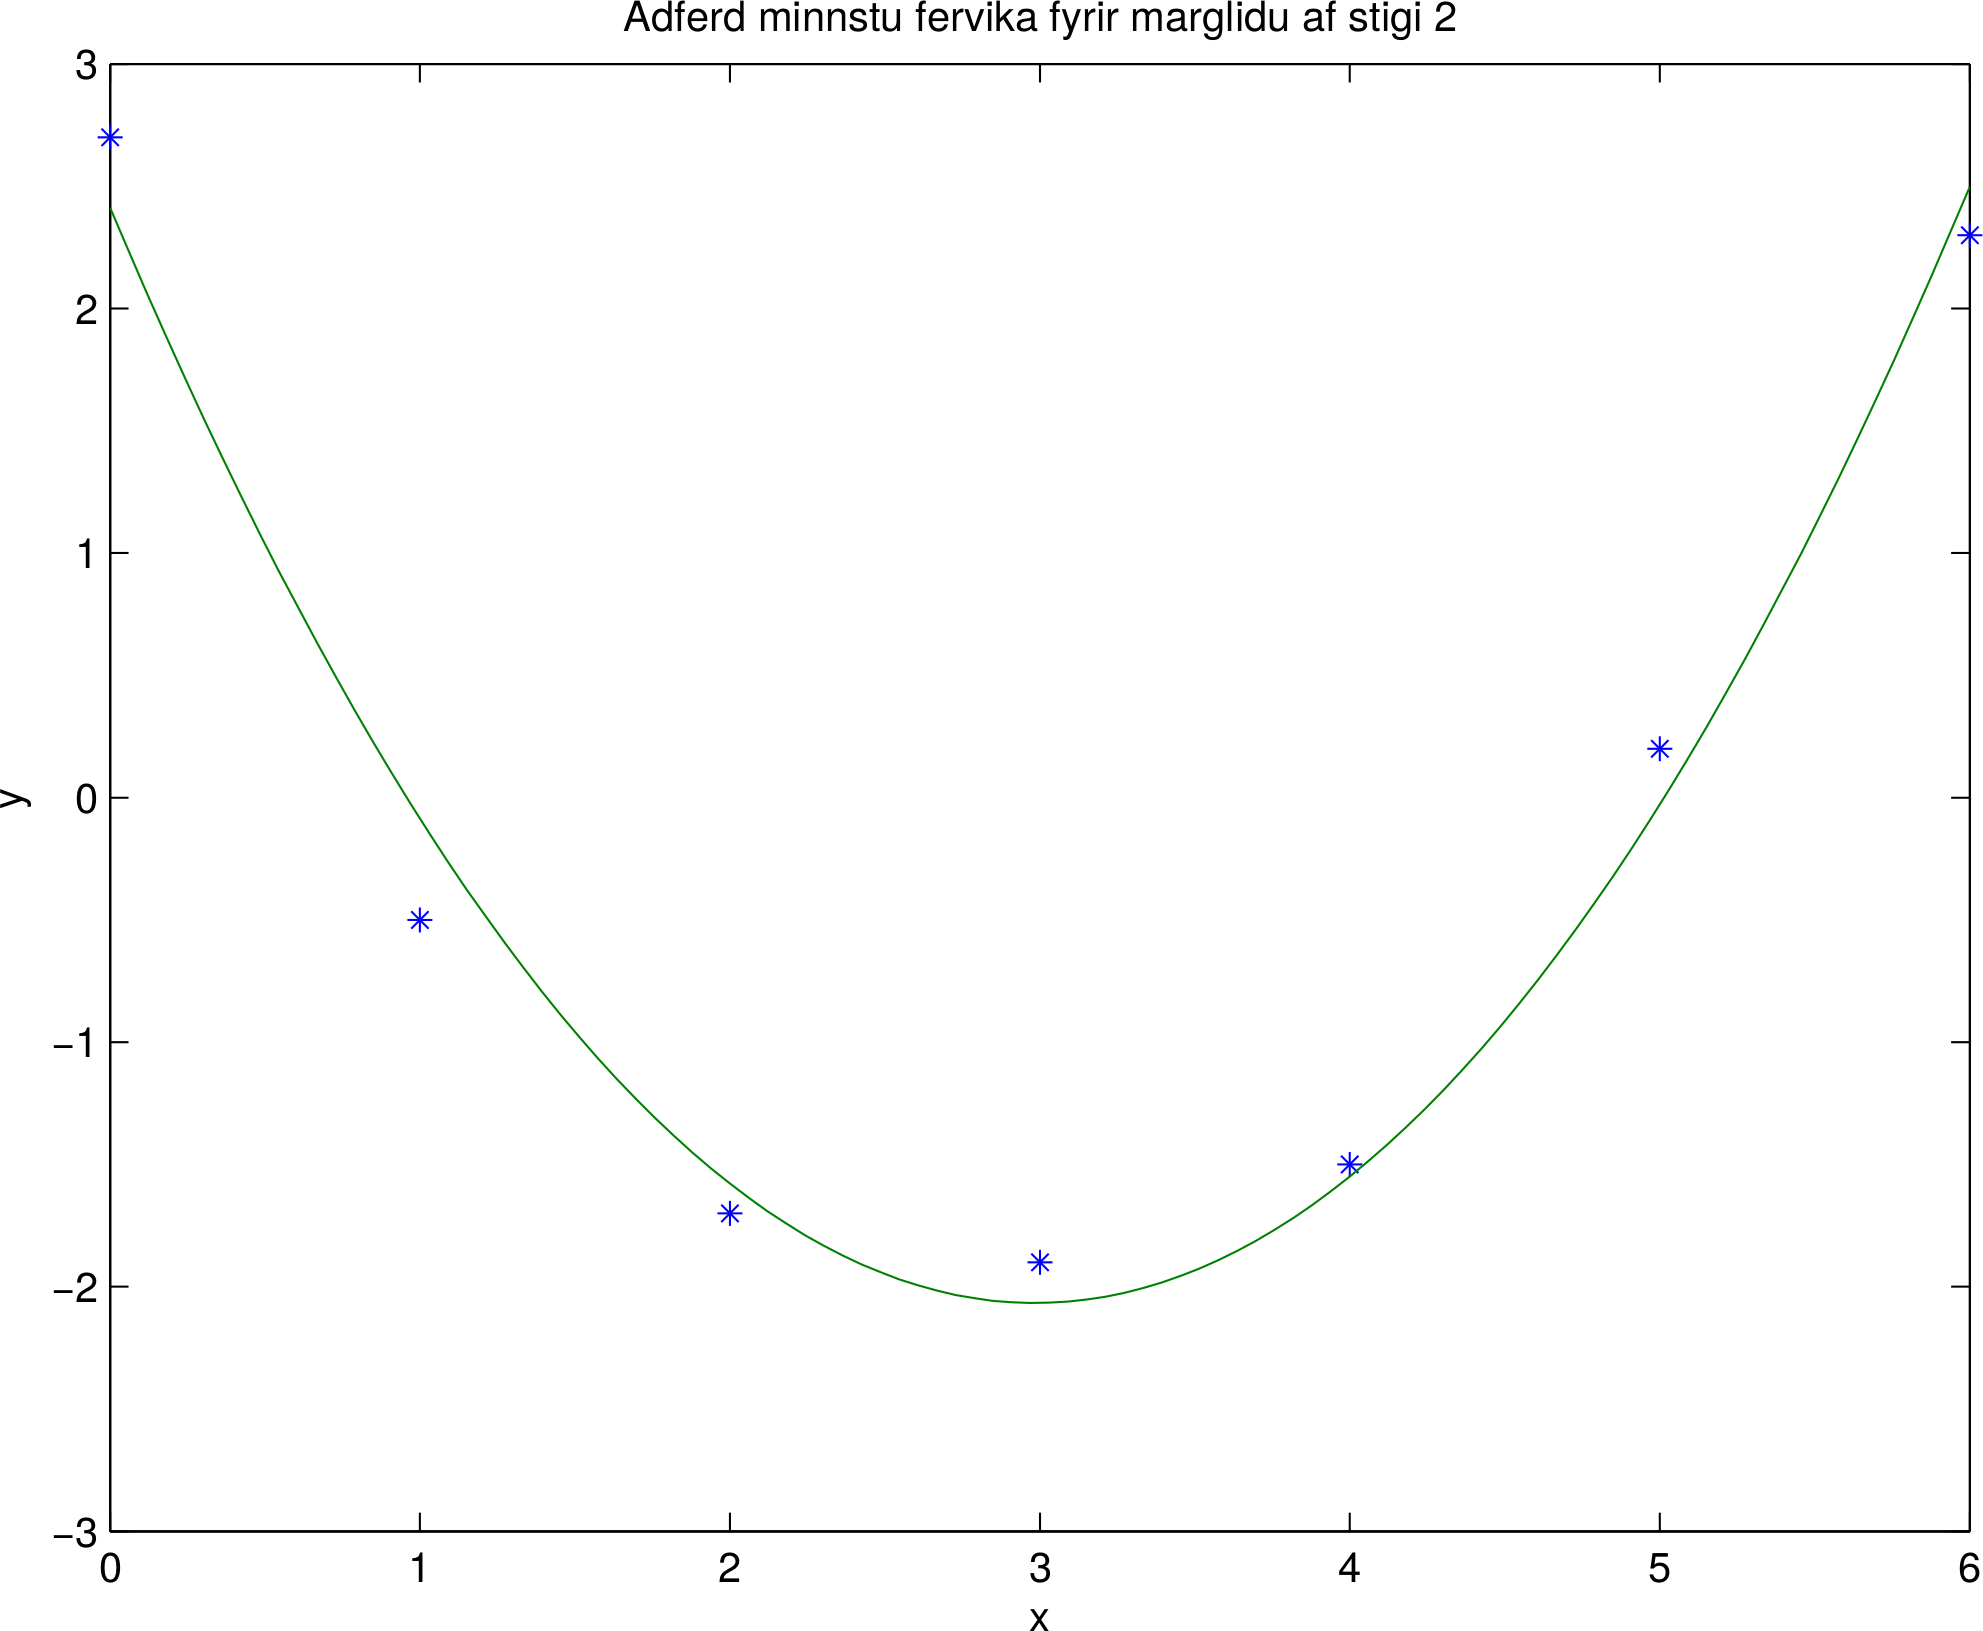
\includegraphics[scale=0.4]{synidaemi_minnstu_fervik}
 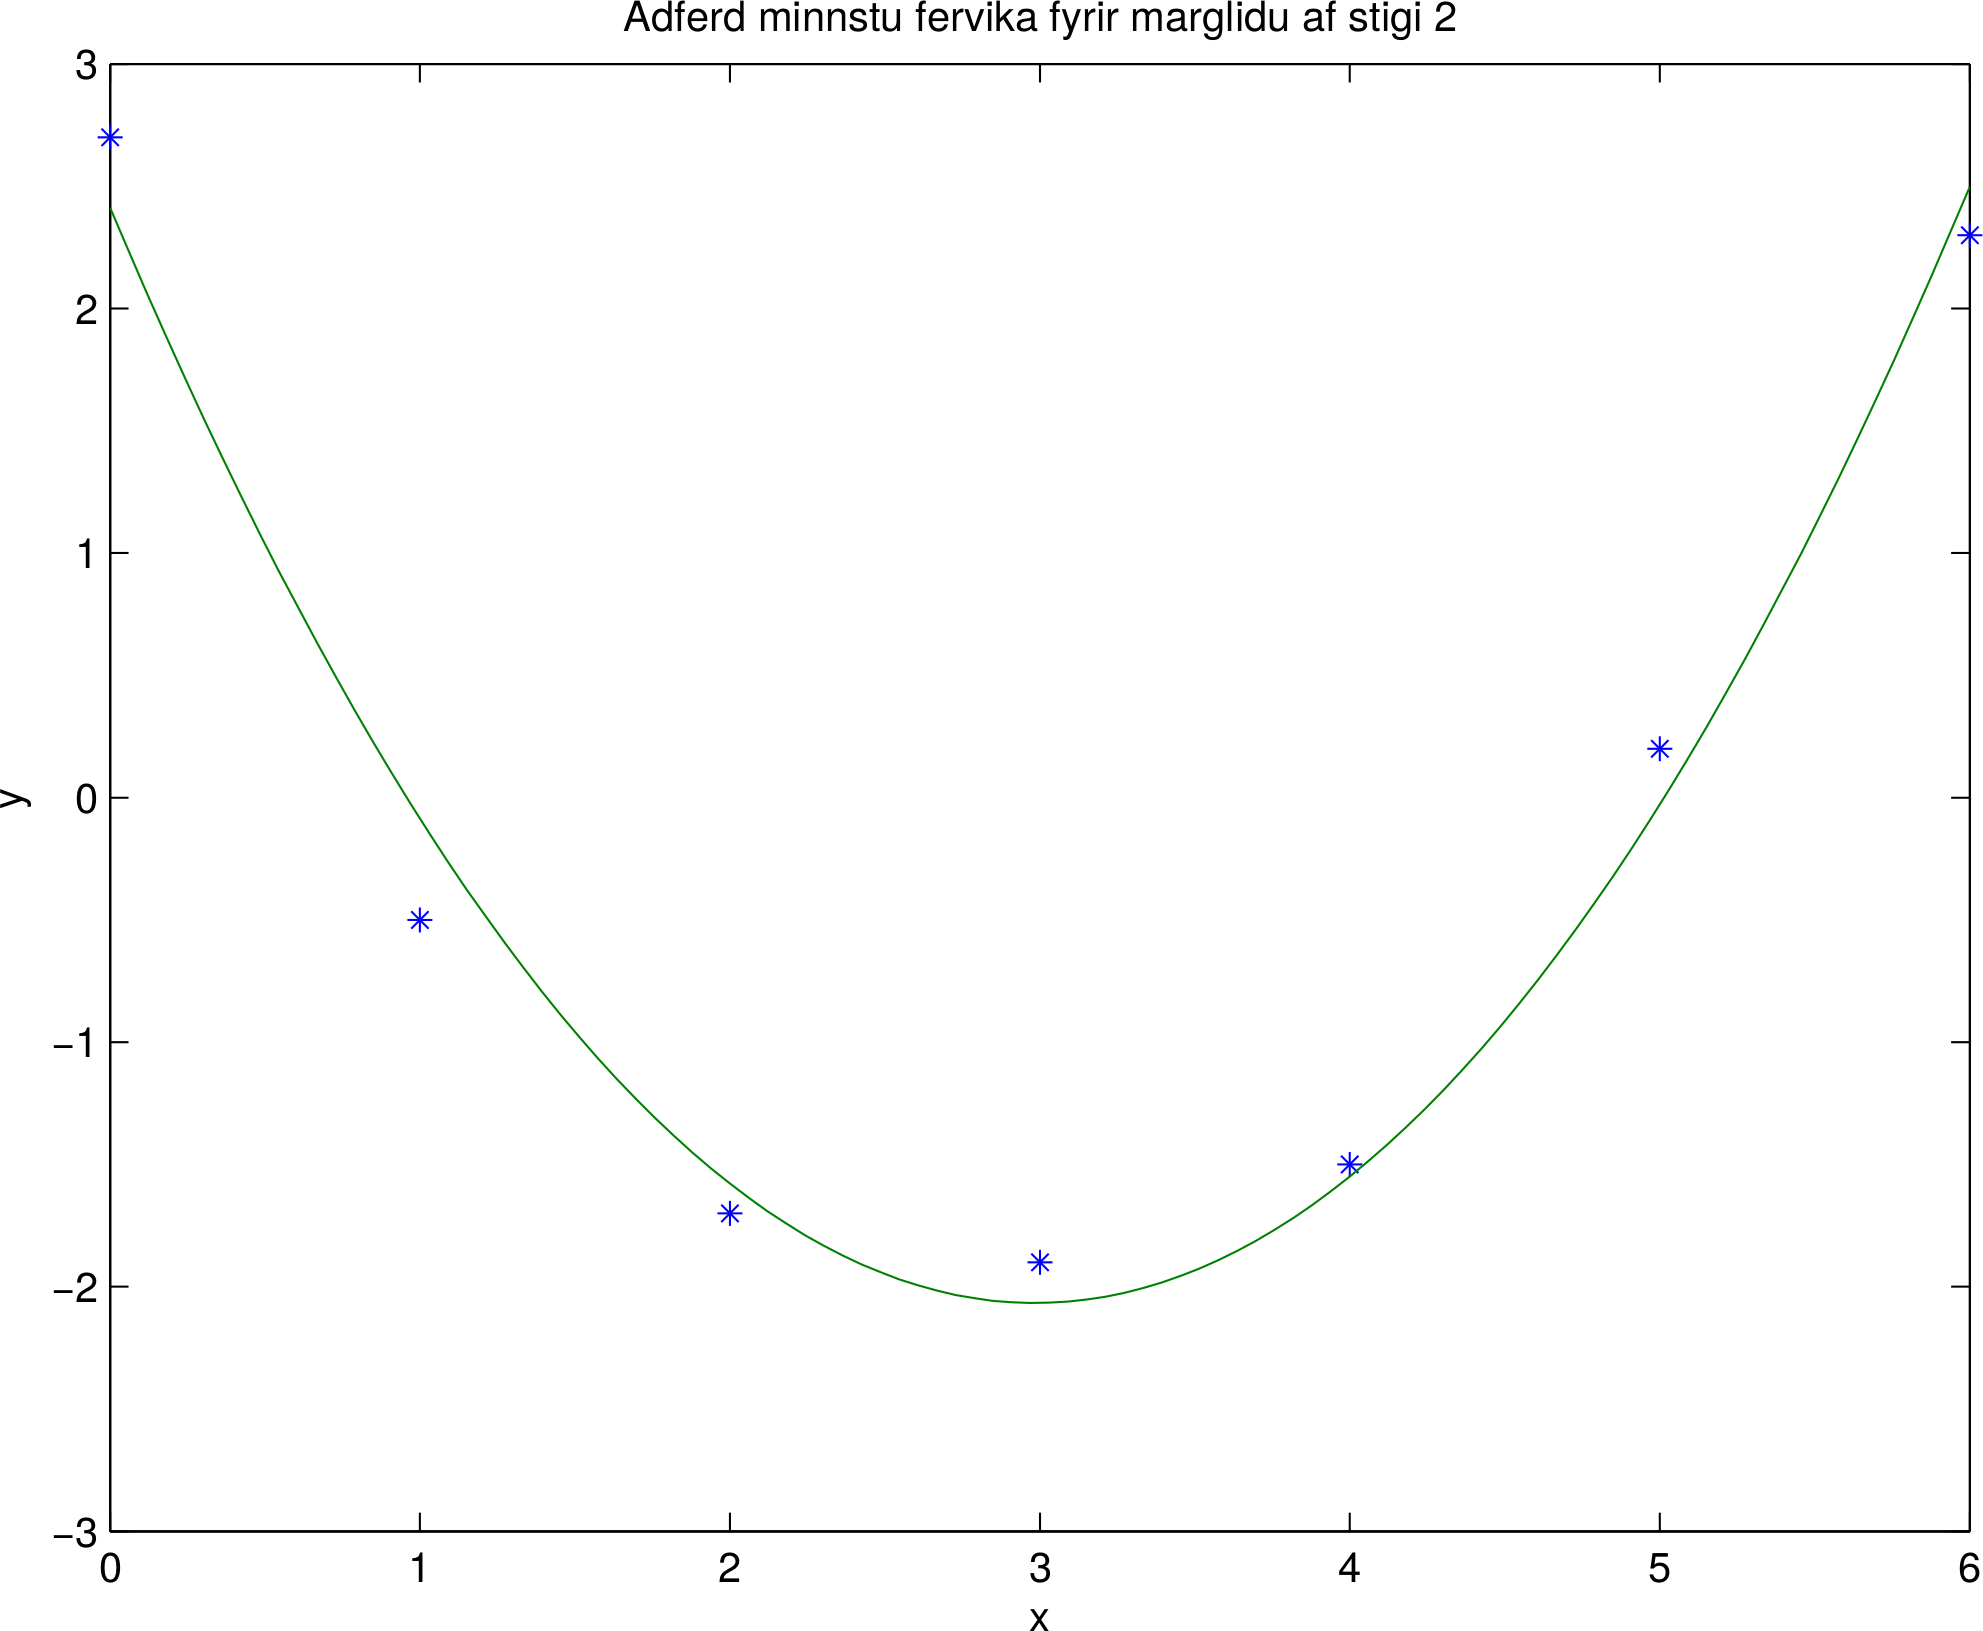
\includegraphics[scale=0.5,clip=true,trim=40 190 40 190]{./synidaemi_minnstu_fervik.pdf}
 \end{center}
\end{frame}

\begin{frame}{Kafli 5: Fræðilegar spurningar}
  \begin{enumerate}
  \item  Hvernig er reiknirit Horners og hver er tilgangur þess?
  \item  Hvernig er brúunarverkefnið fyrir punktana 
$(x_0,y_0),\dots,(x_m,y_m)$?
  \item  Rökstyðjið að einungis sé til ein brúunarmargliða 
af stigi $\leq m$ fyrir 
brúunarpunktana $(x_0,y_0),\dots,(x_m,y_m)$
  \item Hvernig er Lagrange form brúunarmargliðu og hvernig eru
    Lagrange-margliður fyrir gefið punktasafn skilgreindar?  
  \item  Hvernig er Newton-form brúunarmargliðu fyrir 
 fyrir punktana $(x_0,y_0),\dots,(x_m,y_m)$ þar sem
$x_i\neq x_j$?
  \item  Hvernig eru mismunakvótarnir $y[x_i,\ldots,x_{i+j}]$
    skilgreindir?
  \item Hvað er alhæft brúunarverkefni? 
  \item Hvernig er margfeldni brúunarpunkts í alhæfðu brúunarverkefni 
skilgreind?
  \item Rökstyðjið að alhæfða brúunarverkefnið með $m+1$ skilyrði
hafi ótvírætt ákvarðaða lausn af stigi $\leq m$.  
  \item  Hvernig er skekkjuformúlan í nálgun á falli $f(x)$ með alhæfðri
    brúunarmargliðu $p(x)$ sett fram með mismunakvótum?
  \end{enumerate}
\end{frame}

\begin{frame}{Kafli 5: Fræðilegar spurningar}
  \begin{enumerate}
  \item [11.]  Hvernig er skekkjuformúlan í nálgun á falli $f(x)$ með alhæfðri
    brúunarmargliðu $p(x)$ sett fram með $m+1$ afleiðu af $f$?
  \item [12.]  Hvaða skilyrði þarf þriðja stigs splæsifall að uppfylla 
og hvað vantar mörg skilyrði upp á að þau gefi ótvírætt ákvarðað fall?
  \item  [13.] Hvernig eru ekki-hnúts endaskilyrði á splæsifalli?
  \item  [14.] Hvernig eru þvinguð endaskilyrði á splæsifalli?
  \item  [15.] Hvernig eru náttúrleg endaskilyrði á splæsifalli?
  \item  [16.] Hvernig eru lotubundin endaskilyrði á splæsifalli?
  \item  [17.] Lýsið því hvernig splæsiferlar eru notaðir til þess að
    teikna ferla í plani.
  \item  [18.] Lýsið aðferð minnstu fervika.  
  \item  [19.] Hvernig er jöfnuhneppið
    sem þarf að leysa í aðferð minnstu fervika?
  \item  [21.] Hvernig er jafna bestu línu gegnum punktasafn fundin?
  \item  [22.] Hvernig er jafna besta fleygboga gegnum punktasafn fundin?
   \end{enumerate}
\end{frame}

\end{document}